\subsection{紧李代数的嘉当子代数}

引理 1. 设 G 是李群，K 是 G 的紧子群，F 是 L(G) 上的不变双线性型。设 \(x, y \in \mathrm{L}(\mathrm{G})\) 。则存在 K 的元素 k，使得 \(\mathrm{F}(u, [(\mathrm{Ad}k)(x), y]) = 0\) 对一切 \(u \in \mathrm{L}(\mathrm{K})\) 成立。

从 K 到 R 的函数 \(v \mapsto \mathrm{F}((\operatorname{Ad} v)(x), y)\) 连续，因而在某点 \(k \in K\) 处取得极小值。设 \(u \in \mathrm{L}(K)\) ，令

\[
h (t) = \mathrm{F} ((\mathrm{Ad} \exp (t u). k) (x), y), \quad t \in \mathbf {R}.
\]

我们有 \(h(t) \geq h(0)\) （对一切 \(t\) ）；此外，由第 III 章 §3 第 12 节命题 44，

\[
\frac {d h}{d t} (0) = \mathrm{F} ([ u, (\mathrm{Ad} k) (x) ], y) = \mathrm{F} (u, [ (\mathrm{Ad} k) (x), y ]),
\]

引理得证（《实变函数》，第 I 章，§1，第 7 节，命题 7）。

定理 1. 设 g 是紧李代数。g 的嘉当子代数（第 VII 章，§2，第 1 节，定义 1）就是它的极大交换子代数；特别地，g 是它的诸嘉当子代数之并。群 \(\operatorname{Int}(\mathfrak{g})\) 传递地作用在 g 的嘉当子代数所成的集上。

由于 g 是约化的，它的嘉当子代数是交换的（第 VII 章，§2，第 4 节，定理 2 的推论 3）。反之，设 t 是 g 的一个交换子代数。由 §1 第 3 节命题 1，对一切 \(x \in t\) ，ad x 是半单的；由第 VII 章，§2，第 3 节，命题 10，存在 g 的包含 t 的嘉当子代数。这就证明了定理的第一个断言。

现设 \(\mathfrak{t}\) 与 \(\mathfrak{t}'\) 是 \(\mathfrak{g}\) 的两个嘉当子代数。我们证明存在 \(u \in \operatorname{Int}(\mathfrak{g})\) 使得 \(u(\mathfrak{t}) = \mathfrak{t}'\) 。由 §1 第 3 节命题 1，可以假定 \(\mathfrak{g}\) 具有 L(G) 的形式，其中 G 是连通紧李群，并且可以在 g 上选取一个分离的不变对称双线性型 F。设 x（相应地，\(x'\) ）是 g 的正则元，使得 \(\mathfrak{t} = \mathfrak{g}^{0}(x)\) （相应地，\(\mathfrak{t}' = \mathfrak{g}^{0}(x')\) ）（第 VII 章，§3，第 3 节，定理 2）。对 K = G 应用引理 1，可见存在 \(k \in G\) 使得 \([(\operatorname{Ad} k)(x), x']\) 关于 F 与 g 正交，从而为零；于是 \((\operatorname{Ad} k)(x) \in \mathfrak{g}^{0}(x') = \mathfrak{t}'\) ，故 \(\mathfrak{g}^{0}((\operatorname{Ad} k)(x)) = \mathfrak{t}'\) ，因为 \((\operatorname{Ad} k)(x)\) 正则。由此得出 \((\operatorname{Ad} k)(\mathfrak{t}) = \mathfrak{t}'\) ，定理得证。

推论. 设 t 与 \(t'\) 是 g 的嘉当子代数，a 是 t 的子集，u 是把 a 变到 \(t'\) 中的 g 的自同构。则存在 \(\text{Int}(\mathfrak{g})\) 的元素 v，使得 \(u \circ v\) 把 t 变到 \(t'\) ，且在 a 上与 u 相合。

令 \(\mathrm{G} = \operatorname{Int}(\mathfrak{g})\) ，并考虑固定子群 \(Z_{\mathrm{G}}(\mathfrak{a})\) ，即 \(\mathfrak{a}\) 在 \(G\) 中的固定子群；这是 \(G\) 的一个李子群，其李代数 \(\mathfrak{z}_{\mathfrak{g}}(\mathfrak{a})\) 由 \(\mathfrak{g}\) 中与 \(\mathfrak{a}\) 的每个元素交换的元素组成（第 III 章，§9，第 3 节，命题 7）。于是 \(t\) 与 \(u^{-1}(t')\) 是紧李代数 \(\mathfrak{z}_{\mathfrak{g}}(\mathfrak{a})\) 的两个嘉当子代数。由定理 1，存在元素 \(v\) 属于 \(Z_{\mathrm{G}}(\mathfrak{a})\) ，使得 \(v(t) = u^{-1}(t')\) ；任何这样的元素都具有所要的性质。

\subsection{极大环面}

设 G 是李群。G 的环面是指 G 的一个闭子群，它本身是一个环面（§1 第 2 节），换言之即任一交换的连通紧子群。G 的环面所成的集按包含关系排序后，其极大元称为 G 的极大环面。

定理 2. 设 G 是连通紧李群。

\begin{enumerate}
\def\labelenumi{\alph{enumi})}
\item
  \(\mathbf{G}\) 的诸极大环面的李代数是 \(\mathrm{L}(\mathrm{G})\) 的嘉当子代数。
\item
  设 \(\mathrm{T}_1\) 与 \(\mathrm{T}_2\) 是 \(\mathbf{G}\) 的两个极大环面。则存在 \(g \in \mathbf{G}\) 使得 \(\mathrm{T}_2 = g\mathrm{T}_1g^{-1}\) 。
\item
  G 是它的诸极大环面之并。
\end{enumerate}

设 t 是 L(G) 的一个嘉当子代数；G 中以 t 为李代数的积分子群是闭的（第 VII 章，§2，第 1 节，命题 4 的推论 4）且交换的（定理 1），因而是 G 的一个环面。若 T 是 G 的极大环面，则其李代数交换，故包含于 L(G) 的某个嘉当子代数（定理 1）。由此可知，G 的极大环面恰是 L(G) 的嘉当子代数所对应的 G 的积分子群，由此得 a)。断言 b) 由定理 1 得出，因为典则同态 G → Int(L(G)) 是满射（第 III 章，§6，第 4 节，命题 10 的推论 4）。

用 X 表示 G 的诸极大环面之并，设 T 是 G 的一个极大环面。连续映射 \((g,t)\mapsto gtg^{-1}\) （从 \(G\times T\) 到 G）的像是 X，因而 X 在 G 中闭；于是，为证 c)，只需证明 X 在 G 中开；由于 X 在内自同构下不变，只需证明对一切 \(a \in \mathrm{T}\) ， \(\mathrm{X}\) 是 \(a\) 的邻域。我们对 \(\mathrm{G}\) 的维数作归纳，并区分两种情形：

\begin{enumerate}
\def\labelenumi{\arabic{enumi})}
\item
  a 不是 G 的中心元。设 H 是 a 在 G 中的中心化子的单位元连通分支；这是 G 的一个异于 G 的连通紧子群，它包含 T，因而包含 a。由于 Ad a 半单（ \(\S1\) ，第 1 节），H 的李代数是 Ad a - 1 的幂零空间；于是由第 VII 章 \(\S4\) 第 2 节命题 4，H 的诸共轭之并 Y 是 a 的邻域。由归纳假设，\(H \subset X\) ，故 \(Y \subset X\) ；从而 X 是 a 的邻域。
\item
  a 是 G 的中心元。只需证明对 L(G) 中一切 x，\(a \exp x\) 属于 X。而 L(G) 的每个元素 x 都属于 G 的某个嘉当子代数（定理 1）；对应的积分子群 T' 包含 \(\exp x\) ；由于它共轭于 T，它包含 a，因而包含 \(a \exp x\) ，此即所要证明的。
\end{enumerate}

推论 1. a) \(\mathbf{G}\) 的指数映射是满射。

\begin{enumerate}
\def\labelenumi{\alph{enumi})}
\setcounter{enumi}{1}
\tightlist
\item
  对一切 \(n \geq 1\) ，映射 \(g \mapsto g^n\) 从 \(\mathbf{G}\) 到其自身是满射。
\end{enumerate}

事实上，\(\exp(\mathrm{L}(\mathrm{G}))\) 包含 G 的所有极大环面，由此得 a)。断言

\begin{enumerate}
\def\labelenumi{\alph{enumi})}
\setcounter{enumi}{1}
\tightlist
\item
  由公式 \((\exp x)^n = \exp nx\)（\(x\) 属于 \(\mathrm{L}(\mathrm{G})\) ）得出。
\end{enumerate}

注 1. 存在紧子集 \(\mathrm{K}\) （含于 \(\mathrm{L}(\mathrm{G})\) ）使得 \(\exp_{\mathrm{G}}(\mathrm{K}) = \mathrm{G}\) 。事实上，若 \(\mathrm{T}\) 是 \(\mathrm{G}\) 的极大环面，则存在紧子集 \(\mathrm{C} \subset \mathrm{L}(\mathrm{T})\) 使得 \(\exp_{\mathrm{T}}(\mathrm{C}) = \mathrm{T}\) ；只需取 \(\mathrm{K} = \bigcup_{g \in \mathrm{G}} (\operatorname{Ad} g)(\mathrm{C})\) 。

推论 2. G 的诸极大环面之交是 G 的中心。

设 x 是 G 的中心的一个元素；由定理 2 c)，存在包含 x 的 G 的极大环面 T；于是 x 属于 T 的所有共轭，从而属于 G 的所有极大环面。反之，若 x 属于 G 的所有极大环面，则由定理 2 c)，x 与 G 的每个元素交换。

推论 3. 设 \(g \in \mathbf{G}\) ，\(\mathbf{C}\) 是它的中心化子。则 \(g\) 属于 \(\mathrm{C}_0\) ；群 \(\mathrm{C}_0\) 是 \(\mathbf{G}\) 的包含 \(g\) 的诸极大环面之并。

存在包含 g 的 G 的极大环面 T（定理 2 c)），它包含于 \(C_{0}\) 。此外，群 \(C_{0}\) 是连通紧李群，因而是它的诸极大环面之并（定理 2 c)）；这些极大环面都包含 g（推论 2），故它们恰是 G 的包含 g 的极大环面。

推论 4. 设 \(g \in G\) 。若 \(g\) 正则（第 VII 章，§4，第 2 节，定义 2），则它属于唯一的极大环面，即其中心化子的单位元连通分支。否则，它属于无穷多个极大环面。

由于 Ad g 半单，Ad g-1 的幂零空间的维数也就是 g 的中心化子 C 的维数。由同前命题 8 与定理 1，g 正则当且仅当 \(C_{0}\) 是 G 的极大环面。结论由推论 3 立即得出。

推论 5. a) 设 S 是 G 的一个环面。S 的中心化子是连通的；它是 G 的包含 S 的诸极大环面之并。

\begin{enumerate}
\def\labelenumi{\alph{enumi})}
\setcounter{enumi}{1}
\tightlist
\item
  设 \(\mathfrak{s}\) 是 \(\mathrm{L}(\mathrm{G})\) 的交换子代数。\(\mathfrak{s}\) 在 \(\mathrm{G}\) 中的固定子群是连通的；它是 \(\mathrm{G}\) 的李代数包含 \(\mathfrak{s}\) 的诸极大环面之并。
\end{enumerate}

为证 \(a\) ，只需证明：若 G 的元素 \(g\) 与 S 交换，则存在 G 的极大环面同时包含 S 与 \(g\) 。设 C 是 \(g\) 的中心化子，则 \(g \in \mathrm{C}_0\) （推论 3）且 \(\mathrm{S} \subset \mathrm{C}_0\) ；若 T 是连通紧李群 \(\mathrm{C}_0\) 的包含 S 的极大环面，则 \(g \in \mathrm{T}\) （推论 2），由此得 \(a\) )。断言 \(b\) ) 由 \(a\) ) 应用于以 \(\mathfrak{s}\) 为李代数的积分子群的闭包得出，依据是第 III 章，§9，第 3 节，命题 9。

\pandocbounded{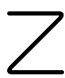
\includegraphics[keepaspectratio]{images/part002_b9f4d066.jpg}}

注 2. 由推论 5 可知，G 的极大环面是极大交换子群。逆命题不真：例如在群 \(\mathbf{SO}(3,\mathbf{R})\) 中，极大环面都是 1 维的，因而不能包含同构于 \((\mathbf{Z}/2\mathbf{Z})^{2}\) 的对角矩阵组成的子群。此外，若 \(g \in \mathbf{SO}(3,\mathbf{R})\) 是非纯量对角矩阵，则 g 是 \(\mathbf{SO}(3,\mathbf{R})\) 的正则元，其中心化子不连通（参见推论 4）。

推论 6. G 的极大环面是自身的中心化子，并且是其李代数的固定子群。

设 T 是 G 的极大环面，C 是它的中心化子；由于 \(L(T)\) 是 \(L(G)\) 的嘉当子代数，我们有 \(L(T) = L(C)\) ，又因 C 连通（推论 5），故 C = T。

推论 7. 设 T 与 T' 是 G 的两个极大环面，A 是 T 的子集，s 是把 A 变到 T' 中的 G 的自同构。则存在 \(g \in G\) 使得 \(s \circ (\operatorname{Int} g)\) 把 T 变到 T' 且在 A 上与 s 相合。

设 C 是 A 的中心化子。则 T 与 \(s^{-1}(T')\) 是 \(C_{0}\) 的两个极大环面；\(C_{0}\) 中满足 \((\operatorname{Int} g)(\mathrm{T}) = s^{-1}(\mathrm{T}')\) 的任何元素 g 都具有所要的性质。

推论 8. 设 H 是紧李群，T 是 H 的极大环面。则 \(\mathrm{H} = \mathrm{N}_{\mathrm{H}}(\mathrm{T}) \cdot \mathrm{H}_{0}\) ，且 \(\mathrm{N}_{\mathrm{H}}(\mathrm{T})\) 到 H 中的单射诱导一个从 \(\mathrm{N}_{\mathrm{H}}(\mathrm{T}) / \mathrm{N}_{\mathrm{H}_{0}}(\mathrm{T})\) 到 \(H/H_{0}\) 上的同构。

设 \(h \in H\) 。则 \(h^{-1}Th\) 是 \(H_0\) 的极大环面，故（定理 2）存在 \(g \in H_0\) 使得 \(hg \in N_H(T)\) ；于是 \(h\) 属于 \(N_H(T).H_0\) ，第一个断言得证。第二个断言立即得证。

注。3) 设 G 是李代数为紧李代数的连通李群。G 的嘉当子群是以 L(G) 的嘉当子代数为李代数的积分子群（连通紧群的嘉当子群因此就是它的极大环面）。如果把处处出现的用语「极大环面」换成「嘉当子群」，定理 2 及其诸推论对 G 仍然成立。这立即由下述事实得出：依据 §1 第 4 节命题 5，G 是向量群 V 与连通紧群 K 的直积，且 G 的嘉当子群是 V 与 K 的极大环面之积。此外，注意由上面的推论 6 可知，G 的嘉当子群也可以定义为 L(G) 的嘉当子代数的固定子群。

* 4) 定理 2 的部分 \(c\) 也可按如下方式证明。给 G 装备一个不变黎曼度量（§1 第 3 节，命题 3）。于是，对 G 的任一元素 \(g\) ，存在通过 \(g\) 与 G 的单位元的极大测地线（Hopf-Rinow 定理），并且可以验证这样一条测地线的闭包是 G 的一个子环面。*

\subsection{子群与商群的极大环面}

命题 1. 设 G 与 G' 是两个连通紧李群。

\begin{enumerate}
\def\labelenumi{\alph{enumi})}
\item
  设 \(f: \mathbf{G} \to \mathbf{G}'\) 是李群满态射。\(\mathbf{G}'\) 的极大环面是在 \(f\) 下 \(\mathbf{G}\) 的诸极大环面的像。若 \(f\) 的核在 \(\mathbf{G}\) 中是中心的（例如是离散的），则 \(\mathbf{G}\) 的极大环面是在 \(f\) 下 \(\mathbf{G}'\) 的诸极大环面的逆像。
\item
  设 \(\mathrm{H}\) 是 \(\mathrm{G}\) 的连通闭子群。\(\mathrm{H}\) 的每个极大环面都是 \(\mathrm{H}\) 与 \(\mathrm{G}\) 的某个极大环面之交。
\item
  设 H 是 G 的连通闭正规子群。H 的极大环面是 G 的极大环面与 H 的交。
\item
  设 T 是 G 的极大环面；则 L(T) 是 L(G) 的嘉当子代数（第 2 节，定理 2 a)），于是 L(f(T)) 是 L(G') 的嘉当子代数（第 VII 章，§2，第 1 节，命题 4 的推论 2）；由此得出 f(T) 是 G' 的极大环面（第 2 节，定理 2 a)）。若 Ker f 含于 G 的中心，则它含于 T（定理 2 的推论 2），故 T = \(f^{-1}(f(T))\) 。
\end{enumerate}

反之，设 \(T'\) 是 \(G'\) 的一个极大环面；我们证明存在 G 的极大环面 T 使得 \(f(\mathrm{T}) = \mathrm{T}'\) 。设 \(T_{1}\) 是 G 的一个极大环面；则 \(f(\mathrm{T}_{1})\) 是 \(G'\) 的极大环面，且存在 \(g' \in G'\) 使得 \(\mathrm{T}' = g' f(\mathrm{T}_{1}) g'^{-1} (\mathrm{Th.~2~b})\) ；若 \(g \in G\) 满足 \(f(g) = g'\) ，则 \(\mathrm{T}' = f(\mathrm{T})\) ，其中 \(\mathrm{T} = g\mathrm{T}_{1}g^{-1}\) 。

\begin{enumerate}
\def\labelenumi{\alph{enumi})}
\setcounter{enumi}{1}
\item
  设 S 是 H 的一个极大环面；它是 G 的环面，故存在包含 S 的 G 的极大环面 T。于是 \(T \cap H\) 是 H 的包含 S 的交换子群，故等于 S（第 2 节，注 2）。
\item
  由 §1 第 3 节命题 2 c)，L(G) 是 L(H) 与一个理想的直积；于是 L(H) 的嘉当子代数是 L(G) 的嘉当子代数与 L(H) 的交。从而对 G 的任一极大环面 T，T∩H 包含 H 的某个极大环面 S，且 S = T∩H（第 2 节，注 2）。
\end{enumerate}

注。1) 命题 1 立即推广到李代数为紧李代数的连通群。特别地，若 G 是李代数为紧李代数的连通李群，则 G 的嘉当子群（参见第 2 节注 3）恰是连通紧李群 Ad(G) 的诸极大环面（在从 G 到 Ad(G) 的典则同态下）的逆像。

\begin{enumerate}
\def\labelenumi{\arabic{enumi})}
\setcounter{enumi}{1}
\tightlist
\item
  设 G 是连通紧李群，\(\widetilde{\mathrm{D}}(\mathrm{G})\) 是群 \(\mathrm{D}(\mathrm{G})\) 的泛覆盖，\(f : \widetilde{\mathrm{D}}(\mathrm{G}) \to \mathrm{G}\) 是从 \(\tilde{\mathrm{D}}(\mathrm{G})\) 到 \(\mathrm{D}(\mathrm{G})\) 与从 \(\mathrm{D}(\mathrm{G})\) 到 G 的典则态射的复合。则映射 \(T \mapsto f^{-1}(\mathrm{T})\) 是从 G 的极大环面集到 \(\tilde{\mathrm{D}}(\mathrm{G})\) 的极大环面集上的双射；逆双射把极大环面 \(\tilde{T}\) （\(\tilde{\mathrm{D}}(\mathrm{G})\) 中的）对应为 G 的极大环面 \(\mathrm{C}(\mathrm{G})_{0}.f(\tilde{\mathrm{T}})\) 。
\end{enumerate}

\subsection{极大秩子群}

我们把连通李群 G 的李代数的秩称为 G 的秩，记作 rk G。由定理 2 a)，连通紧李群的秩是其诸极大环面的公共维数。

设 G 是连通紧李群，H 是 G 的闭子群。若 H 连通，则 \(rkH \leq rkG\) （因为 H 的极大环面是 G 中的环面）。由定理 2 c)，说 H 连通且为极大秩（即为秩 rkG），就等于说 H 是 G 的某些极大环面之并。我们立即由命题 1 推出：

命题 2. 设 \(f: \mathrm{G} \to \mathrm{G}'\) 是核为中心的连通紧李群满态射。映射 \(\mathrm{H} \mapsto f(\mathrm{H})\) 与 \(\mathrm{H}' \mapsto f^{-1}(\mathrm{H}')\) 是 \(\mathrm{G}\) 的极大秩连通闭子群集与 \(\mathrm{G}'\) 的相应子群集之间的互逆双射。

命题 3. 设 G 是连通紧李群，H 是极大秩连通闭子群。

\begin{enumerate}
\def\labelenumi{\alph{enumi})}
\item
  紧流形 G/H 是单连通的。
\item
  由 H 到 G 中的典则单射诱导的同态 \(\pi_1(\mathrm{H})\to \pi_1(\mathrm{G})\) 是满射。
\end{enumerate}

由于 H 连通，我们有正合列（《一般拓扑学》，第 XI 章，编写中）

\[
\pi_ {1} (\mathrm{H}) \rightarrow \pi_ {1} (\mathrm{G}) \rightarrow \pi_ {1} (\mathrm{G/H}, \bar {e}) \rightarrow 0
\]

其中 \(\bar{e}\) 是 G 的单位元在 G/H 中的像。由于 G/H 连通，这立即给出断言 a) 与 b) 的等价性。此外，若 \(f : G' \to G\) 是核为中心的连通紧李群满态射，则对 G 证明本命题（取 a) 的形式）与对 \(G'\) 证明它是一回事（命题 2）。于是，我们可以先把 G 换成 \(\text{Ad}(G)\) ，再假定 G 半单，然后通过把 G 换成一个泛覆盖（ \(\S1\) ，第 4 节，命题 4 的推论 2），假定 G 单连通。但此时断言 b) 是平凡的。

命题 4. 设 G 是紧李群，H 是 G 的极大秩连通闭子群，N 是 H 在 G 中的正规化子。则 H 在 N 中指数有限，且是 N 的单位元连通分支。

事实上，H 的李代数包含 L(G) 的一个嘉当子代数。于是，由第 VII 章，§2，第 1 节，命题 4 的推论 4，H 是 N 的单位元连通分支。由于 N 紧，H 在 N 中指数有限。

注。1) 满足 rkH = rkG 的 G 的每个积分子群 H 都是闭的：事实上，前面的证明表明 H 是其正规化子的单位元连通分支，而该正规化子是 G 的闭子群。

\begin{enumerate}
\def\labelenumi{\arabic{enumi})}
\setcounter{enumi}{1}
\tightlist
\item
  采用命题 4 的记号，每个闭子群 \(H'\) （G 中包含 H 且使 \((H':H)\) 有限者）都正规化 H，故含于 N；同样，\(H'\) 的正规化子也含于 N。特别地，N 是自身的正规化子。
\end{enumerate}

\subsection{Weyl 群}

设 G 是连通紧李群，T 是 G 的极大环面。用 \(N_{G}(T)\) 表示 T 在 G 中的正规化子；由第 4 节命题 4，商群 \(N_{G}(T)/T\) 有限。我们把它记作 \(W_{G}(T)\) 或 \(W(T)\) ，称之为 G 的极大环面 T 的 Weyl 群，或 G 相对于 T 的 Weyl 群。由于 T 交换，\(N_{G}(T)\) 经 G 的内自同构在 T 上的作用过渡到商，便得到群 \(W_{G}(T)\) 在李群 T 上的一个作用，称为典则作用。由第 2 节定理 2 的推论 6，这个作用是忠实的：相伴的同态 \(W_{G}(T) \rightarrow Aut T\) 是单射。

若 \(T'\) 是 G 的另一个极大环面，且 \(g \in G\) 使得 Int g 把 T 映为 \(T'\) （第 2 节，定理 2 b)），则 Int g 诱导一个同构 \(a_g\) （从 \(\mathrm{W}_{\mathrm{G}}(\mathrm{T})\) 到 \(\mathrm{W}_{\mathrm{G}}(\mathrm{T}')\) ），并且 \(a_g(s)(gtg^{-1}) = gs(t)g^{-1}\) 对一切 \(s \in \mathrm{W}_{\mathrm{G}}(\mathrm{T})\) 与一切 \(t \in T\) 成立。

命题 5. a) G 的每个共轭类都与 T 相交。

\begin{enumerate}
\def\labelenumi{\alph{enumi})}
\setcounter{enumi}{1}
\tightlist
\item
  \(\mathrm{T}\) 与 \(\mathbf{G}\) 的诸共轭类的交是 Weyl 群的轨道。
\end{enumerate}

设 \(g \in \mathbf{G}\) ；由第 2 节定理 2，存在 \(h \in \mathbf{G}\) 使得 \(g \in h\mathrm{Th}^{-1}\) ，由此得 \(a\) )。由 Weyl 群的定义，\(\mathrm{W_G(T)}\) 在 \(T\) 上同一轨道中的任两个元素在 \(G\) 中共轭；反之，设 \(a, b\) 是 \(T\) 的两个在 \(G\) 中共轭的元素。存在 \(h \in G\) 使得 \(b = hah^{-1}\) ；对 \(A = \{a\}\) 、\(s = \operatorname{Int} h\) 、\(T' = T\) 应用第 2 节定理 2 的推论 7，可见存在 \(g \in G\) 使得 \(\operatorname{Int} hg\) 把 \(T\) 映到 \(T\) 且把 \(a\) 映到 \(b\) 。于是 \(hg\) 在 \(\mathrm{W_G(T)}\) 中的类把 \(a\) 映到 \(b\) ，命题得证。

推论 1. T 到 G 中的典则单射经过渡到商，定义一个从 \(\mathrm{T}/\mathrm{W}_{\mathrm{G}}(\mathrm{T})\) 到 G 的共轭类空间 \(\mathrm{G}/\mathrm{Int}(\mathrm{G})\) 上的同胚。

事实上，这是两个紧空间之间的连续双射（参见《一般拓扑学》，第 III 章，第 29 页，推论 1）。

推论 2. 设 E 是 G 的在内自同构下稳定的子集。则 E 在 G 中开（相应地，闭、稠密）当且仅当 \(E \cap T\) 在 T 中开（相应地，闭、稠密）。

这由推论 1 以及典则映射 \(T \rightarrow T/W_{G}(T)\) 与 \(G \rightarrow G/Int(G)\) 是开映射得出（《一般拓扑学》，第 III 章，第 10 页，引理 2）。

用 g 表示 G 的李代数，用 t 表示 T 的李代数。\(W_{\mathrm{G}}(\mathrm{T})\) 在 T 上的作用诱导出群 \(W_{\mathrm{G}}(\mathrm{T})\) 在 R-向量空间 t 上的一个表示，称为典则表示。

命题 6. a) G 在 g 上（对伴随表示而言）的每条轨道都与 t 相交。

\begin{enumerate}
\def\labelenumi{\alph{enumi})}
\setcounter{enumi}{1}
\tightlist
\item
  \(\mathfrak{t}\) 与 \(\mathrm{G}\) 的诸轨道的交是 \(\mathrm{W_G(T)}\) 在 \(\mathfrak{t}\) 上的轨道。
\end{enumerate}

断言 \(a\) ) 由第 1 节定理 1 得出。设 \(x, y\) 是 \(\mathfrak{t}\) 的两个在 \(\operatorname{Ad}(\mathrm{G})\) 下共轭的元素，\(h \in \mathrm{G}\) 满足 \((\operatorname{Ad} h)(x) = y\) 。对 \(\mathfrak{a} = \{x\}\) 、\(u = \operatorname{Ad} h, \mathfrak{t}' = \mathfrak{t}\) 应用第 1 节定理 1 的推论，可见存在 \(g \in \mathrm{G}\) 使得 \(\operatorname{Ad} hg\) 把 \(\mathfrak{t}\) 映到 \(\mathfrak{t}\) 且把 \(x\) 映到 \(y\) 。于是 \(hg \in \mathrm{N}_{\mathrm{G}}(\mathrm{T})\) （第 III 章，§9，第 4 节，命题 11），且 \(hg\) 在 \(\mathrm{W}_{\mathrm{G}}(\mathrm{T})\) 中的类把 \(x\) 映到 \(y\) ，命题得证。

推论. t 到 g 中的典则单射经过渡到商，定义一个从 \(\mathfrak{t}/\mathrm{W}_{\mathrm{G}}(\mathrm{T})\) 到 \(\mathfrak{g}/\mathrm{Ad}(\mathrm{G})\) 上的同胚。

把这个映射记作 \(j\) ；它是双射且连续（命题 6）。我们有交换图式

\[
\begin{array}{c c c} \mathfrak {t} & \stackrel {{i}} {{\longrightarrow}} & \mathfrak {g} \\ p \Big \downarrow & & \Big \downarrow q \\ \mathfrak {t} / \mathrm{W} _ {\mathrm{G}} (\mathrm{T}) & \stackrel {{j}} {{\longrightarrow}} & \mathfrak {g} / \mathrm{Ad} (\mathrm{G}) \end{array}
\]

其中 p 与 q 是商映射，i 是典则单射。由于 i 与 q 是真的（《一般拓扑学》，第 I 章，§10，第 1 节，命题 2，及《一般拓扑学》，第 III 章，§4，第 1 节，命题 2 c)），且 p 是满射，由此得出 j 是真的（《一般拓扑学》，第 I 章，§10，第 1 节，命题 5），从而是同胚。

命题 7. 设 H 是 G 的包含 T 的闭子群。

\begin{enumerate}
\def\labelenumi{\alph{enumi})}
\item
  用 \(\mathrm{W}_{\mathrm{H}}(\mathrm{T})\) 表示子群 \(\mathrm{N}_{\mathrm{H}}(\mathrm{T})/\mathrm{T}\) （\(\mathrm{W}_{\mathrm{G}}(\mathrm{T})\) 中的）；群 \(H/H_{0}\) 同构于商群 \(\mathrm{W}_{\mathrm{H}}(\mathrm{T})/\mathrm{W}_{\mathrm{H}_{0}}(\mathrm{T})\) 。
\item
  H 连通当且仅当 \(\mathrm{W}_{\mathrm{G}}(\mathrm{T})\) 中在 H 有代表的每个元素都属于 \(\mathrm{W}_{\mathrm{H}_{0}}(\mathrm{T})\) 。
\end{enumerate}

断言 \(a\) ) 由第 2 节定理 2 的推论 8 得出，而断言 \(b\) ) 是 \(a\) ) 的一个特殊情形。

\subsection{极大环面与同态的提升}

设 G 是连通紧李群，T 是 G 的极大环面。考虑 G 的换位子群 \(\mathrm{D}(\mathrm{G})\) 及其泛覆盖 \(\tilde{\mathrm{D}}(\mathrm{G})\) ；设 \(p: \tilde{\mathrm{D}}(\mathrm{G}) \to \mathrm{G}\) 是典则态射 \(\tilde{\mathrm{D}}(\mathrm{G}) \to \mathrm{D}(\mathrm{G})\) 与 \(\mathrm{D}(\mathrm{G}) \to \mathrm{G}\) 的复合。则 \(\tilde{\mathrm{D}}(\mathrm{G})\) 是连通紧李群（ \(\S1\) ，第 4 节，命题 4 的推论 2）；此外，T 在 p 下的逆像 \(\tilde{T}\) 是 \(\tilde{\mathrm{D}}(\mathrm{G})\) 的极大环面（第 3 节，命题 1）。

引理 2. 设 H 是李群，\(f_{\mathrm{T}}: \mathrm{T} \to \mathrm{H}\) 与 \(\tilde{f}: \tilde{\mathrm{D}}(\mathrm{G}) \to \mathrm{H}\) 是李群态射，满足 \(f_{\mathrm{T}}(p(t)) = \tilde{f}(t)\) 对一切 \(t \in \tilde{\mathrm{T}}\) 成立。则存在唯一的李群态射 \(f: \mathrm{G} \to \mathrm{H}\) 使得 \(f \circ p = \tilde{f}\) ，且 \(f\) 在 \(\mathrm{T}\) 上的限制为 \(f_{\mathrm{T}}\) 。

令 \(Z = \mathrm{C}(\mathrm{G})_{0}\) ；由 §1 第 4 节命题 4 的推论 1，李群态射 \(g: Z \times \tilde{\mathrm{D}}(\mathrm{G}) \to \mathrm{G}\) （它满足 \(g(z, x) = z^{-1} p(x)\) ）是一个覆盖；它的核由偶 \((z, x)\) （满足 \(p(x) = z\) ）组成，对这些偶有 \(x \in p^{-1}(\mathrm{Z}) \subset \tilde{\mathrm{T}}\) 。由于态射 \((z, x) \mapsto f_{\mathrm{T}}(z^{-1}) \tilde{f}(x)\) （从 \(Z \times \tilde{\mathrm{D}}(\mathrm{G})\) 到 H）把 \(\operatorname{Ker} g\) 映为 \(\{e\}\) ，故存在从 G 到 H 的态射 f 使得 \(f \circ p = \tilde{f}\) 且 \(f(z) = f_{\mathrm{T}}(z)\) 对 \(z \in Z\) 成立。也有 \(f(t) = f_{\mathrm{T}}(t)\) 对 \(t \in p(\tilde{\mathrm{T}})\) 成立；由于 \(T = Z.p(\tilde{\mathrm{T}})\) ，f 在 T 上的限制确为 \(f_{T}\) 。

命题 8. 设 G 是连通紧李群，T 是 G 的极大环面，H 是李群，\(\varphi : \mathrm{L}(\mathrm{G}) \to \mathrm{L}(\mathrm{H})\) 是李代数同态。则存在李群态射 \(f: \mathrm{G} \to \mathrm{H}\) 满足 \(\mathrm{L}(f) = \varphi\) ，当且仅当存在李群态射 \(f_{\mathrm{T}}: \mathrm{T} \to \mathrm{H}\) 满足 \(\mathrm{L}(f_{\mathrm{T}}) = \varphi | \mathrm{L}(\mathrm{T})\) ；此时 \(f_{\mathrm{T}} = f | \mathrm{T}\) 。

若 \(f: \mathrm{G} \to \mathrm{H}\) 是满足 \(\mathrm{L}(f) = \varphi\) 的李群态射，则限制 \(f_{\mathrm{T}}\) （即 \(f\) 在 \(\mathrm{T}\) 上的限制）是从 \(\mathrm{T}\) 到 \(\mathrm{H}\) 的唯一满足 \(\mathrm{L}(f_{\mathrm{T}}) = \varphi | \mathrm{L}(\mathrm{T})\) 的态射。反之，设 \(f_{\mathrm{T}}: \mathrm{T} \to \mathrm{H}\) 是满足 \(\mathrm{L}(f_{\mathrm{T}}) = \varphi | \mathrm{L}(\mathrm{T})\) 的李群态射。设 \(\tilde{\mathrm{D}}(\mathrm{G})\) 与 \(p\) 如上；映射 \(\mathrm{L}(p)\) 诱导一个从 \(\mathrm{L}(\tilde{\mathrm{D}}(\mathrm{G}))\) 到导代数 \(\mathfrak{b}\) （\(\mathrm{L}(\mathrm{G})\) 的）上的同构。存在李群态射 \(\tilde{f}: \tilde{\mathrm{D}}(\mathrm{G}) \to \mathrm{H}\) 使得 \(\mathrm{L}(\tilde{f}) = (\varphi | \mathfrak{b}) \circ \mathrm{L}(p)\) （第 III 章，§6，第 1 节，定理 1）。态射 \(t \mapsto \tilde{f}(t)\) 与 \(t \mapsto f_{\mathrm{T}}(p(t))\) （都是从 \(\tilde{\mathrm{T}}\) 到 \(\mathrm{H}\) ）诱导相同的李代数同态，因而相合。应用引理 2，我们推出存在态射 \(f: \mathrm{G} \to \mathrm{H}\) 使得 \(\mathrm{L}(f)\) 与 \(\varphi\) 在 \(\mathrm{L}(\mathrm{T})\) 与 \(\mathfrak{b}\) 上相合。由于 \(\mathrm{L}(\mathrm{G}) = \mathfrak{b} + \mathrm{L}(\mathrm{T})\) ，我们有 \(\mathrm{L}(f) = \varphi\) 。

命题 9. 设 G 是连通紧李群，T 是 G 的极大环面，H 是李群，\(f: G \to H\) 是态射。则 f 单射当且仅当它在 T 上的限制单射。

事实上，由第 2 节定理 2，G 的正规子群 \(\mathrm{Ker}f\) 约化为单位元当且仅当它与 T 的交约化为单位元。

\section{复半单李代数的紧形式}

\subsection{实形式}

若 \(\mathfrak{a}\) 是复李代数，我们用 \(\mathfrak{a}_{[\mathbf{R} ]}\) （有时也简记为 \(\mathfrak{a}\) ）表示由标量限制得到的实李代数。若 \(\mathfrak{g}\) 是实李代数，我们用 \(\mathfrak{g}_{(\mathbf{C})}\) （有时也简记为 \(\mathfrak{g}_{\mathbf{C}}\) ）表示由标量扩张得到的复李代数 \(\mathbf{C}\otimes_{\mathbf{R}}\mathfrak{g}\) 。实李代数同态 \(\mathfrak{g}\to \mathfrak{a}_{[\mathbf{R}]}\) 与复李代数同态 \(\mathfrak{g}_{(\mathbf{C})}\to \mathfrak{a}\) 成一一对应：若 \(f:\mathfrak{g}\to \mathfrak{a}_{[\mathbf{R}]}\) 与 \(g:\mathfrak{g}_{(\mathbf{C})}\to \mathfrak{a}\) 相对应，则 \(f(x) = g(1\otimes x)\) 且 \(g(\lambda \otimes x) = \lambda f(x)\) 对 \(x\in \mathfrak{g},\lambda \in \mathbf{C}\) 成立。

定义 1. 设 \(\mathfrak{a}\) 是复李代数。\(\mathfrak{a}\) 的实形式是指实子代数 \(\mathfrak{g}\) （\(\mathfrak{a}\) 的），它是一个 \(\mathbf{R}\) -结构（在 \(\mathbf{C}\) -向量空间 \(\mathfrak{a}\) 上）（《代数学》，第 II 章，§8，第 1 节，定义 1）。

这就是说，复李代数同态 \(\mathfrak{g}_{(\mathbf{C})}\to\mathfrak{a}\) （与典则单射 \(g\to a_{[R]}\) 相伴）是双射。于是，a 的实子代数 g 是 a 的实形式，当且仅当实向量空间 a 的子空间 g 与 ig 互为余补。a 相对于实形式 g 的共轭是满足下式的映射 \(\sigma:a\to a\)

\[
\sigma (x + i y) = x - i y, \quad x, y \in \mathfrak {g}.\tag{1}
\]

命题 1. a) 设 \(\mathfrak{g}\) 是 \(\mathfrak{a}\) 的实形式，\(\sigma\) 是 \(\mathfrak{a}\) 相对于 \(\mathfrak{g}\) 的共轭。则：

\[
\sigma^ {2} = \mathrm{Id} _ {\mathfrak {a}}, \quad \sigma (\lambda x + \mu y) = \bar {\lambda} \sigma (x) + \bar {\mu} \sigma (y), \quad [ \sigma (x), \sigma (y) ] = \sigma [ x, y ]\tag{2}
\]

其中 \(\lambda, \mu \in \mathbf{C}\) ，\(x, y \in \mathfrak{a}\) 。元素 \(x\) （\(\mathfrak{a}\) 中的）属于 \(\mathfrak{g}\) 当且仅当 \(\sigma(x) = x\) 。b) 设 \(\sigma: \mathfrak{a} \to \mathfrak{a}\) 是满足 (2) 的映射。则不动点所成的集 \(\mathfrak{g}\) （\(\sigma\) 的）是 \(\mathfrak{a}\) 的实形式，且 \(\sigma\) 是 \(\mathfrak{a}\) 相对于 \(\mathfrak{g}\) 的共轭。

证明是直接的。

注意，若 B 表示 a 的 Killing 型，且 g 是 a 的实形式，则 B 在 g 上的限制是 g 的 Killing 型；特别地，B 在 \(g \times g\) 上取实值。假定 a 约化；则实李代数 g 紧当且仅当 B 在 g 上的限制是负的（§1 第 3 节）。这时我们称 g 是 a 的紧实形式。

\subsection{对应于谢瓦莱系的实形式}

在本节中，我们考虑分裂半单李代数 \((\mathfrak{a},\mathfrak{h})\) （域 \(\mathbf{C}\) 上的；第 VIII 章，§2，第 1 节），其根系为 \(\mathrm{R}(\mathfrak{a},\mathfrak{h}) = \mathrm{R}\) ，以及一个谢瓦莱系 \((X_{\alpha})_{\alpha \in \mathbb{R}}\) （\((\mathfrak{a},\mathfrak{h})\) 的）（第 VIII 章，§2，第 4 节，定义 3）。

回忆（同前），线性映射 \(\theta: a \to a\) ——在 h 上与 \(-Id_{h}\) 相合，且把 \(X_{\alpha}\) 映为 \(X_{-\alpha}\) （对一切 \(\alpha \in R\) ）——是 a 的自同构。此外（同前，命题 7），若 \(\alpha, \beta, \alpha + \beta\) 都是根，则

\[
[ X _ {\alpha}, X _ {\beta} ] = \mathrm{N} _ {\alpha , \beta} X _ {\alpha + \beta}\tag{3}
\]

其中 \(\mathrm{N}_{\alpha ,\beta}\in \mathbf{R}^*\) ，且

\[
\mathrm{N} _ {- \alpha , - \beta} = \mathrm{N} _ {\alpha , \beta}.\tag{4}
\]

用 \(\mathfrak{h}_0\) 表示 \(\mathfrak{h}\) 的由 \(H\in \mathfrak{h}\) （满足 \(\alpha (H)\in \mathbf{R}\) 对一切 \(\alpha \in \mathbb{R}\) ）组成的实向量子空间。则 \(\mathfrak{h}_0\) 是一个 \(\mathbf{R}\) -结构（在复向量空间 \(\mathfrak{h}\) 上），且 \([X_{\alpha},X_{-\alpha}]\in \mathfrak{h}_0\) 对一切 \(\alpha \in \mathbb{R}\) 成立，而 \(\mathfrak{a}\) 的 Killing 型 B 在 \(\mathfrak{h}_0\) 上的限制是分离的正型（第 VIII 章，§2，第 2 节，注 2）。此外，

\[
\mathrm{B} (H, X _ {\alpha}) = 0, \quad \mathrm{B} (X _ {\alpha}, X _ {\beta}) = 0 \text {if} \alpha + \beta \neq 0, \quad \mathrm{B} (X _ {\alpha}, X _ {- \alpha}) <   0\tag{5}
\]

（第 VIII 章，§2，第 2 节，命题 1，及第 4 节，引理 3）。

命题 2. a) 实向量子空间 \(\mathfrak{a}_0 = \mathfrak{h}_0 + \sum_{\alpha \in \mathrm{R}} \mathbf{R}X_\alpha\) （\(\mathfrak{a}\) 的）是 \(\mathfrak{a}\) 的实形式，\(\mathfrak{h}_0\) 是它的嘉当子代数。偶 \((\mathfrak{a}_0, \mathfrak{h}_0)\) 是分裂半单实李代数，\((X_\alpha)\) 是它的谢瓦莱系。

\begin{enumerate}
\def\labelenumi{\alph{enumi})}
\setcounter{enumi}{1}
\tightlist
\item
  设 \(\sigma\) 是 \(\mathfrak{a}\) 相对于 \(\mathfrak{a}_0\) 的共轭。则 \(\sigma \circ \theta = \theta \circ \sigma\) 。\(\sigma \circ \theta\) 的不动点所成的集是一个紧实形式 \(\mathfrak{a}_u\) （\(\mathfrak{a}\) 的），\(i\mathfrak{h}_0\) 是它的嘉当子代数。
\end{enumerate}

部分 a) 由前文立即得出。我们证明 b)。由于 \(\sigma\circ\theta\) 与 \(\theta\circ\sigma\) 是从 a 到 a 的两个在 \(a_{0}\) 上相合的半线性映射，它们相合。而 \(\sigma\circ\theta\) 满足第 1 节的条件 (2)，故它是 a 相对于实形式 \(a_{u}\) 的共轭，该实形式由 \(x\in a\) （满足 \(\sigma\circ\theta(x)=x\) 者）组成（命题 1）。对一切 \(\alpha\in R\) ，令

\[
u _ {\alpha} = X _ {\alpha} + X _ {- \alpha}, v _ {\alpha} = i (X _ {\alpha} - X _ {- \alpha}).\tag{6}
\]

则 R-向量空间 \(a_{u}\) 由 \(ih_{0}\) 、诸 \(u_{\alpha}\) 与诸 \(v_{\alpha}\) 生成。更确切地说，若选取 R 的一个房 C，则

\[
\mathfrak {a} _ {u} = i \mathfrak {h} _ {0} \oplus \bigoplus_ {\alpha \in \mathrm{R} _ {+} (\mathrm{C})} \left(\mathbf {R} u _ {\alpha} + \mathbf {R} v _ {\alpha}\right).\tag{7}
\]

显然 \(i\mathfrak{h}_0\) 是 \(\mathfrak{a}_u\) 的嘉当子代数，余下要证 \(B\) 在 \(\mathfrak{a}_u\) 上的限制是负的。而 \(i\mathfrak{h}_0\) 与诸形如 \(\mathbf{R}u_{\alpha}\oplus \mathbf{R}v_{\alpha}\) 的子空间关于 B 两两正交，此由 (5) 得知；B 在 \(i\mathfrak{h}_0\) 上的限制是负的，且

\[
\mathrm{B} (u _ {\alpha}, u _ {\alpha}) = \mathrm{B} (v _ {\alpha}, v _ {\alpha}) = 2 \mathrm{B} (X _ {\alpha}, X _ {- \alpha}) <   0, \quad \mathrm{B} (u _ {\alpha}, v _ {\alpha}) = 0,\tag{8}
\]

由此即得结论。

注. 采用前面的记号，我们有下列公式：

\[
[ h, u _ {\alpha} ] = - i \alpha (h) v _ {\alpha}, [ h, v _ {\alpha} ] = i \alpha (h) u _ {\alpha}, [ u _ {\alpha}, v _ {\alpha} ] = 2 i H _ {\alpha}, (h \in \mathfrak {h})\tag{9}
\]

\[
[ u _ {\alpha}, u _ {\beta} ] = \mathrm{N} _ {\alpha , \beta} u _ {\alpha + \beta} + \mathrm{N} _ {\alpha , - \beta} u _ {\alpha - \beta}, \quad \alpha \neq \pm \beta ,\tag{10}
\]

\[
[ v _ {\alpha}, v _ {\beta} ] = - \mathrm{N} _ {\alpha , \beta} u _ {\alpha + \beta} + \mathrm{N} _ {\alpha , - \beta} u _ {\alpha - \beta}, \quad \alpha \neq \pm \beta ,\tag{11}
\]

\[
[ u _ {\alpha}, v _ {\beta} ] = \mathrm{N} _ {\alpha , \beta} v _ {\alpha + \beta} - \mathrm{N} _ {\alpha , - \beta} v _ {\alpha - \beta}, \quad \alpha \neq \pm \beta ,\tag{12}
\]

（在后三个公式中，按惯例约定 \(\mathrm{N}_{\gamma, \delta} = 0\) 当 \(\gamma + \delta\) 不是根时）。

注意 \(\sum \mathbf{R}u_{\alpha}\) 是 \(\mathfrak{a}\) 的实子代数，即 \(\mathfrak{a}_0 \cap \mathfrak{a}_u\) 。

设 \(\mathrm{Q}(\mathrm{R})\) 是 R 的根权格（第 VI 章，§1，第 9 节）。回忆：对每个同态 \(\gamma : \mathrm{Q}(\mathrm{R}) \to \mathbf{C}^*\) ，对应着初等自同构 \(f(\gamma)\) （\(\mathfrak{a}\) 的），满足 \(f(\gamma)(h) = h\) 对一切 \(h \in \mathfrak{h}\) ，且 \(f(\gamma)X_{\alpha} = \gamma(\alpha)X_{\alpha}\) （第 VIII 章，§5，第 2 节）。

命题 3. 设 \(\mathfrak{g}\) 是 \(\mathfrak{a}\) 的紧实形式，满足 \(\mathfrak{g} \cap \mathfrak{h} = i\mathfrak{h}_0\) 。则存在同态 \(\gamma: \mathrm{Q}(\mathrm{R}) \to \mathbf{R}_{+}^{*}\) 使得 \(\mathfrak{g} = f(\gamma)(\mathfrak{a}_u)\) 。

设 \(\tau\) 是 \(\mathfrak{a}\) 相对于 \(\mathfrak{g}\) 的共轭。由假设，\(\tau(x) = x\) 对 \(x \in i\mathfrak{h}_0\) 成立，故 \(\tau(x) = -x\) 对 \(x \in \mathfrak{h}_0\) 成立。于是，对一切 \(\alpha \in \mathrm{R}\) 与一切 \(h \in \mathfrak{h}_0\) ，

\[
[ h, \tau (X _ {\alpha}) ] = [ - \tau (h), \tau (X _ {\alpha}) ] = - \tau ([ h, X _ {\alpha} ]) = - \tau (\alpha (h) X _ {\alpha});
\]

由此得出 \([h, \tau(X_{\alpha})] = -\alpha(h)\tau(X_{\alpha})\) 对一切 \(h \in \mathfrak{h}_0\) 成立，从而对一切 \(h \in \mathfrak{h}\) 亦然。故存在 \(c_{\alpha} \in \mathbf{C}^*\) 使得 \(\tau(X_{\alpha}) = c_{\alpha}X_{-\alpha}\) 。由于 \([X_{\alpha}, X_{-\alpha}] \in \mathfrak{h}_0\) ，我们有 \([\tau(X_{\alpha}), \tau(X_{-\alpha})] = -[X_{\alpha}, X_{-\alpha}]\) ，故 \(c_{\alpha}c_{-\alpha} = 1\) ；同样，公式 (3) 与 (4) 给出 \(c_{\alpha + \beta} = c_{\alpha}c_{\beta}\) 当 \(\alpha, \beta, \alpha + \beta\) 都是根时。由第 VI 章，§1，第 6 节，命题 19 的推论 2，存在同态 \(\delta: \mathrm{Q}(\mathrm{R}) \to \mathbf{C}^*\) 使得 \(\delta(\alpha) = c_{\alpha}\) 对一切 \(\alpha \in \mathrm{R}\) 成立。

现在证明每个 \(c_{\alpha}\) 都严格正。事实上，\(c_{\alpha}\mathrm{B}(X_{\alpha},X_{-\alpha})=\mathrm{B}(X_{\alpha},\tau(X_{\alpha}))\) ，由于 \(\mathrm{B}(X_{\alpha},X_{-\alpha})\) 是负的，只需证明对 a 的每个非零元素 z 有 \(\mathrm{B}(z,\tau(z))<0\) ；而 a 的每个元素都可写成 \(x+iy\) ，其中 x 与 y 属于 g，且

\[
\mathrm{B} (x + i y, \tau (x + i y)) = \mathrm{B} (x + i y, x - i y) = \mathrm{B} (x, x) + \mathrm{B} (y, y),
\]

由假设 B 在 g 上的限制是负的且分离的，故所述断言得证。

由此得出同态 \(\delta\) 取值于 \(\mathbf{R}_+^*\) ；于是存在同态 \(\gamma : \mathrm{Q}(\mathrm{R}) \to \mathbf{R}_+^*\) 使得 \(\delta = \gamma^{-2}\) 。此时 \(f(\gamma)^{-1}(\mathfrak{g})\) 是 \(\mathfrak{a}\) 的实形式；对应的共轭为 \(\tau' = f(\gamma)^{-1} \circ \tau \circ f(\gamma)\) 。对一切 \(\alpha \in \mathbb{R}\) ，我们有

\[
\tau^ {\prime} (X _ {\alpha}) = f (\gamma) ^ {- 1} (\tau (c _ {\alpha} ^ {- 1 / 2} X _ {\alpha})) = f (\gamma) ^ {- 1} (c _ {\alpha} ^ {1 / 2} X _ {- \alpha}) = X _ {- \alpha},
\]

且 \(\tau'(h) = \tau(h) = h\) 对 \(h \in i\mathfrak{h}_0\) 成立；由此得出 \(\tau'\) 是相对于 \(\mathfrak{a}_u\) 的共轭，从而 \(f(\gamma)^{-1}(\mathfrak{g}) = \mathfrak{a}_u\) 。

\subsection{紧形式的共轭性}

定理 1. 设 \(\mathfrak{a}\) 是复半单李代数。

\begin{enumerate}
\def\labelenumi{\alph{enumi})}
\item
  \(\mathfrak{a}\) 有紧（相应地，可分裂）实形式。
\item
  群 \(\operatorname{Int}(\mathfrak{a})\) 传递地作用在 a 的紧（相应地，可分裂）实形式所成的集上。
\end{enumerate}

设 \(\mathfrak{h}\) 是 \(\mathfrak{a}\) 的一个嘉当子代数。则 \((\mathfrak{a},\mathfrak{h})\) 是分裂的（第 VIII 章，§2，第 1 节，注 2），并且有一个谢瓦莱系 \((X_{\alpha})\) （第 VIII 章，§4，第 4 节，命题 5 的推论）。部分 \(a)\) 于是由命题 2 得出。设 \(\mathfrak{g}\) 是 \(\mathfrak{a}\) 的紧实形式；我们证明存在 \(v\in\mathrm{Int}(\mathfrak{a})\) 使得 \(v(\mathfrak{a}_{u})=\mathfrak{g}\) 。设 \(\mathfrak{t}\) 是 \(\mathfrak{g}\) 的一个嘉当子代数；则 \(\mathfrak{t}_{(\mathbf{C})}\) 是 \(\mathfrak{a}\) 的嘉当子代数；由于 \(\mathrm{Int}(\mathfrak{a})\) 传递地作用在 \(\mathfrak{a}\) 的嘉当子代数所成的集上（第 VII 章，§3，第 2 节，定理 1），我们可化到 \(\mathfrak{t}_{(\mathbf{C})}=\mathfrak{h}\) 的情形。由于 \(\mathfrak{g}\) 是紧形式，自同态 ad \(h\) （\(h\in\mathfrak{t}\) ）的特征值都是纯虚的（ \(\S1\) ，第 3 节，命题 1），故根 \(\alpha\in\mathbb{R}\) 把 \(\mathfrak{t}\) 映到 \(i\mathbf{R}\) 中；这就蕴含 \(\mathfrak{t}=i\mathfrak{h}_{0}\) 。于是由第 2 节命题 3，存在 \(v\in\mathrm{Int}(\mathfrak{a})\) 使得 \(v(\mathfrak{a}_{u})=\mathfrak{g}\) ，从而在紧形式的情形得到 \(b)\)。最后，设 \(\mathfrak{m}_{1}\) 与 \(\mathfrak{m}_{2}\) 是 \(\mathfrak{a}\) 的两个可分裂实形式。存在标架 \((\mathfrak{m}_{1},\mathfrak{h}_{1},\mathrm{B}_{1},(X_{\alpha}^{1}))\) 与 \((\mathfrak{m}_{2},\mathfrak{h}_{2},\mathrm{B}_{2},(X_{\alpha}^{2}))\) （第 VIII 章，§4，第 1 节）。它们以显然的方式扩张成基 \(e_{1}\) 与 \(e_{2}\) （\(\mathfrak{a}\) 的）。\(\mathfrak{a}\) 的把 \(e_{1}\) 映为 \(e_{2}\) 的自同构把 \(\mathfrak{m}_{1}\) 映为 \(\mathfrak{m}_{2}\) ；于是，只需应用第 VIII 章 §5 第 3 节命题 5，便得到存在元素 \(u\) （属于 \(\mathrm{Aut}_{0}(\mathfrak{a})=\mathrm{Int}(\mathfrak{a})\) ）使得 \(u(\mathfrak{m}_{1})=\mathfrak{m}_{2}\) 。

注. 我们将在很后面给出复半单李代数的实形式的一般分类。

推论 1. 设 \(\mathfrak{g}\) 与 \(\mathfrak{g}'\) 是两个紧实李代数。则 \(\mathfrak{g}\) 与 \(\mathfrak{g}'\) 同构当且仅当复李代数 \(\mathfrak{g}_{(\mathbf{C})}\) 与 \(\mathfrak{g}'_{(\mathbf{C})}\) 同构。

条件显然是必要的。反之，假定 \(\mathfrak{g}_{(\mathbf{C})}\) 与 \(\mathfrak{g}'_{(\mathbf{C})}\) 同构。设 c（相应地，\(c'\) ）是 g（相应地，\(g'\) ）的中心，s（相应地，\(s'\) ）是 g（相应地，\(g'\) ）的导代数。则 \(\mathfrak{c}_{(\mathbf{C})}\) 与 \(\mathfrak{c}'_{(\mathbf{C})}\) 分别是 \(\mathfrak{g}_{(\mathbf{C})}\) 与 \(\mathfrak{g}'_{(\mathbf{C})}\) 的中心，因而同构；由此得出交换代数 c 与 \(c'\) 同构。同样，\(\mathfrak{s}_{(\mathbf{C})}\) 与 \(\mathfrak{s}'_{(\mathbf{C})}\) 同构，故 s 与 \(s'\) ——它们是两个同构的复半单李代数的紧实形式——由定理 1 b) 得知同构。

推论 2. 设 \(\mathfrak{a}\) 是复李代数。下列条件等价：

\begin{enumerate}
\def\labelenumi{(\roman{enumi})}
\item
  \(\mathfrak{a}\) 是约化的。
\item
  存在紧实李代数 \(\mathfrak{g}\) 使得 \(\mathfrak{a}\) 同构于 \(\mathfrak{g}(\mathbf{C})\) 。
\item
  存在紧李群 \(\mathbf{G}\) 使得 \(\mathfrak{a}\) 同构于 \(\mathrm{L}(\mathrm{G})_{(\mathbf{C})}\) 。
\end{enumerate}

由 §1 第 3 节定义 1，条件 (ii) 与 (iii) 等价且蕴含 (i)。若 \(\mathfrak{a}\) 约化，则它是一个交换代数（它显然有紧实形式）与一个半单代数（由定理 1 \(a\) ) 它有紧实形式）的直积，故 (i) 蕴含 (ii)。

推论 3. 设 \(\mathfrak{a}_1\) 与 \(\mathfrak{a}_2\) 是两个复半单李代数。\(\mathfrak{a}_1 \times \mathfrak{a}_2\) 的紧实形式是诸积 \(\mathfrak{g}_1 \times \mathfrak{g}_2\) ，其中对 \(i = 1, 2\) ，\(\mathfrak{g}_i\) 是 \(\mathfrak{a}_i\) 的紧实形式。

事实上，存在紧实形式 \(g_{1}\) （相应地，\(g_{2}\) ）——\(a_{1}\) （相应地，\(a_{2}\) ）的——；于是 \(g_{1} \times g_{2}\) 是 \(a_{1} \times a_{2}\) 的紧实形式。把定理 1 b) 应用于 \(a_{1}, a_{2}\) 与 \(a_{1} \times a_{2}\) ，即得本推论。

注意，由上面的推论 3 可知，紧实李代数 g 单当且仅当复李代数 \(\mathfrak{g}_{(\mathbf{C})}\) 单。我们说 g 是 \(A_{n}\) 型、或 \(B_{n}, \ldots\) 型的，如果 \(\mathfrak{g}_{(\mathbf{C})}\) 是 \(A_{n}\) 型、或 \(B_{n}, \ldots\) 型的（第 VIII 章，§2，第 2 节）。由上面的推论 1，两个紧单实李代数同构当且仅当它们同型。

设 G 是概单连通紧李群（第 III 章，§9，第 8 节，定义 3）。我们说 G 是 \(A_{n}\) 型、或 \(B_{n}\) 型、\ldots，如果 G 的李代数是 \(A_{n}\) 型、或 \(B_{n}\) 型、\ldots。两个单连通概单紧李群同构当且仅当它们同型。

\subsection{\texorpdfstring{例 I：\(A_{n}\) 型紧李代数}{例 I：A\_\{n\} 型紧李代数}}

设 V 是有限维复向量空间，\(\Phi\) 是 V 上分离的正埃尔米特型。与 \(\Phi\) 相伴的酉群（参见《代数学》，第 IX 章）是子群 \(\mathbf{U}(\Phi)\) （\(\mathbf{GL}(V)\) 中由复希尔伯特空间 \((V,\Phi)\) 的自同构组成的）；这是群 \(\mathbf{GL}(V)\) 的一个（实）李子群，其李代数是子代数 \(\mathfrak{u}(\Phi)\) （实李代数 \(\mathfrak{gl}(V)\) 中由满足 \(x^{*} = -x\) 的 V 的自同态 x 组成的）（第 III 章，§3，第 10 节，命题 37 的推论 2），其中 \(x^{*}\) 表示 x 相对于 \(\Phi\) 的伴随。由于群 \(\mathbf{U}(\Phi)\) 紧（§1 第 1 节），\(\mathfrak{u}(\Phi)\) 是紧实李代数。同样，特殊酉群 \(\mathbf{SU}(\Phi) = \mathbf{U}(\Phi) \cap \mathbf{SL}(V)\) 是 \(\mathbf{SL}(V)\) 的紧李子群，其李代数为 \(\mathfrak{su}(\Phi) = \mathfrak{u}(\Phi) \cap \mathfrak{sl}(V)\) 。

当 \(V = C^{n}\) 且 \(\varPhi\) 是通常的埃尔米特型（\(C^{n}\) 的典则基关于它标准正交）时，我们把 \(\mathbf{U}(n, \mathbf{C})\) 、\(\mathbf{SU}(n, \mathbf{C})\) 、\(\mathfrak{u}(n, \mathbf{C})\) 、\(\mathfrak{s}\mathfrak{u}(n, \mathbf{C})\) 分别写作 \(\mathbf{U}(\varPhi)\) 、\(\mathbf{SU}(\varPhi)\) 、\(\mathfrak{u}(\varPhi)\) 、\(\mathfrak{s}\mathfrak{u}(\varPhi)\) 。\(\mathbf{U}(n, \mathbf{C})\)（相应地，\(\mathfrak{u}(n, \mathbf{C})\)）的元素

是矩阵 \(A \in \mathrm{M}_{n}(\mathbf{C})\) （满足 \(A.^{t}\bar{A} = I_{n}\) ，相应地 \(A = -^{t}\bar{A}\) ），分别称为酉的（相应地，反埃尔米特的）。

命题 4. a) 复李代数 \(\mathfrak{sl}(V)\) 的紧实形式是诸代数 \(\mathfrak{su}(\Phi)\) ，其中 \(\Phi\) 取遍复向量空间 \(V\) 上分离的正埃尔米特型所成的集。

\begin{enumerate}
\def\labelenumi{\alph{enumi})}
\setcounter{enumi}{1}
\tightlist
\item
  诸代数 \(\mathfrak{u}(\varPhi)\) 是 \(\mathfrak{gl}(\mathrm{V})\) 的紧实形式。
\end{enumerate}

设 \(\varPhi\) 是 V 上分离的正埃尔米特型。对一切 \(x\in\mathfrak{gl}(V)\) ，令 \(\sigma(x)=-x^{*}\) （其中 \(x^{*}\) 是 \(x\) 相对于 \(\varPhi\) 的伴随）。则 \(\sigma\) 满足第 1 节命题 1 的条件 (2)，故不动点集 \(\mathfrak{u}(\varPhi)\) （相应地，\(\mathfrak{su}(\varPhi)\) ）——即 \(\sigma\) 在 \(\mathfrak{gl}(V)\) （相应地，\(\mathfrak{sl}(V)\) ）上的不动点所成的集——是 \(\mathfrak{gl}(V)\) （相应地，\(\mathfrak{sl}(V)\) ）的紧实形式。由于 \(\mathbf{GL}(V)\) 传递地作用在 V 上分离的正埃尔米特型所成的集上（《代数学》，第 IX 章），也传递地作用在 \(\mathfrak{sl}(V)\) 的紧实形式所成的集上（第 3 节，定理 1，及第 VIII 章，§13，第 1 节 (VII)），命题 4 得证。

推论. \(\mathrm{A}_n\) 型（ \(n \geq 1\) ）的每个紧单实李代数同构于 \(\mathfrak{su}(n + 1, \mathbf{C})\) 。

事实上，每个 \(\mathbf{A}_n\) 型复李代数都同构于 \(\mathfrak{sl}(n + 1,\mathbf{C})\) （第 VIII 章，§13，第 1 节）。

注。1) 我们有 \(\mathfrak{gl}(\mathrm{V}) = \mathfrak{sl}(\mathrm{V}) \times \mathbf{C}.1_{\mathrm{V}}\) ，\(\mathfrak{u}(\varPhi) = \mathfrak{su}(\varPhi) \times \mathbf{R}.i1_{\mathrm{V}}\) ；\(\mathfrak{gl}(\mathrm{V})\) 的紧实形式是诸 \(\mathfrak{su}(\varPhi) \times \mathbf{R}. \alpha 1_{\mathrm{V}}, \alpha \in \mathbf{C}^*\) 。

\begin{enumerate}
\def\labelenumi{\arabic{enumi})}
\setcounter{enumi}{1}
\tightlist
\item
  若复李代数 \(\mathfrak{a} = \mathfrak{sl}(n,\mathbf{C})\) 装备了第 VIII 章 §13 第 1 节 (IX) 中引入的分裂与谢瓦莱系，则采用第 2 节的记号，
\end{enumerate}

\[
\mathfrak {a} _ {u} = \mathfrak {s u} (n, \mathbf {C}), \quad \mathfrak {a} _ {0} = \mathfrak {s l} (n, \mathbf {R}), \quad \mathfrak {a} _ {u} \cap \mathfrak {a} _ {0} = \mathfrak {o} (n, \mathbf {R}).
\]

\subsection{\texorpdfstring{例 II：\(\mathbf{B}_n\) 型与 \(\mathbf{D}_n\) 型紧李代数}{例 II：\textbackslash mathbf\{B\}\_n 型与 \textbackslash mathbf\{D\}\_n 型紧李代数}}

设 V 是有限维实向量空间，Q 是 V 上分离的正二次型。与 Q 相伴的正交群（《代数学》，第 IX 章）是子群 \(\mathbf{O}(\mathbf{Q})\) （\(\mathbf{GL}(\mathbf{V})\) 中由实希尔伯特空间 (V, Q) 的自同构组成的）；这是 \(\mathbf{GL}(\mathbf{V})\) 的李子群，其李代数是子代数 \(\mathfrak{o}(\mathbf{Q})\) （\(\mathfrak{gl}(\mathbf{V})\) 中由满足 \(x^{*} = -x\) 的 V 的自同态 x 组成的）（第 III 章，§3，第 10 节，命题 37 的推论 2），其中 \(x^{*}\) 表示 x 相对于 Q 的伴随。由于群 \(\mathbf{O}(\mathbf{Q})\) 紧，\(\mathfrak{o}(\mathbf{Q})\) 是紧实李代数。令 \(\mathbf{SO}(\mathbf{Q}) = \mathbf{O}(\mathbf{Q}) \cap \mathbf{SL}(\mathbf{V})\) ；这是 \(\mathbf{O}(\mathbf{Q})\) 的有限指数闭子群（当 dim V ≠ 0 时指数为 2），因而也以 \(\mathfrak{o}(\mathbf{Q})\) 为李代数。

当 \(V = R^{n}\) 且 Q 是通常的二次型（\(R^{n}\) 的典则基关于它标准正交）时，我们把 \(\mathbf{O}(n, \mathbf{R})\) 、\(\mathbf{SO}(n, \mathbf{R})\) 、\(\mathfrak{o}(n, \mathbf{R})\) 分别写作 \(\mathbf{O}(\mathbf{Q})\) 、\(\mathbf{SO}(\mathbf{Q})\) 、\(\mathfrak{o}(\mathbf{Q})\) 。\(\mathbf{O}(n, \mathbf{R})\)（相应地，\(\mathfrak{o}(n, \mathbf{R})\)）的元素

是矩阵 \(A \in \mathrm{M}_n(\mathbf{R})\) （满足 \(A.^t A = I_n\) ，相应地 \(A = -^t A\) ），分别称为正交的（相应地，反对称的）。

设 \(\mathrm{V}_{(\mathbf{C})}\) 是与 \(\mathrm{V}\) 相伴的复向量空间，\(\mathrm{Q}_{(\mathbf{C})}\) 是 \(\mathrm{V}_{(\mathbf{C})}\) 上与 \(\mathbf{Q}\) 相伴的二次型。把 \(\mathfrak{gl}(\mathrm{V})_{(\mathbf{C})}\) 与 \(\mathfrak{gl}(\mathrm{V}_{(\mathbf{C})})\) 等同起来；则 \(\mathfrak{o}(\mathrm{Q})_{(\mathbf{C})}\) 与 \(\mathfrak{o}(\mathrm{Q}_{(\mathbf{C})})\) 等同：这一点是显然的，因为映射 \(x \mapsto x^{*} + x\) （从 \(\mathfrak{gl}(\mathrm{V}_{(\mathbf{C})})\) 到其自身的）是 \(\mathbf{C}\) -线性的。由于 \(\mathfrak{o}(\mathrm{Q}_{(\mathbf{C})})\) 是 \(\mathrm{B}_n\) 型的（当 \(\dim V = 2n + 1\) 、\(n \geq 1\) 时），而是 \(\mathrm{D}_n\) 型的（当 \(\dim V = 2n\) 、\(n \geq 3\) 时）（第 VIII 章，§13，第 2 节与第 4 节），我们推出：

命题 5. \(B_{n}\) 型（\(n \geq 1\) ）、相应地 \(D_{n}\) 型（\(n \geq 3\) ）的每个紧单实李代数，同构于 \(\mathfrak{o}(2n + 1, \mathbf{R})\) 、相应地 \(\mathfrak{o}(2n, \mathbf{R})\) 。

\subsection{秩 1 紧群}

由《一般拓扑学》第 VIII 章 §1 第 4 节命题 3、命题 4 与注 4，拓扑群 \(\mathbf{SU}(2,\mathbf{C})\) 同构于范数为 1 的四元数组成的拓扑群 \(\mathbf{S}_3\) ，且 \(\mathbf{SU}(2,\mathbf{C})\) 关于由矩阵 \(I_2\) 与 \(-I_2\) 组成的子群 Z 的商同构于拓扑群 \(\mathbf{SO}(3,\mathbf{R})\) 。注意 Z 是 \(\mathbf{SU}(2,\mathbf{C})\) 的中心：事实上，由于 \(\mathbf{H} = \mathbf{R}.\mathbf{S}_3\) ，群 \(\mathbf{S}_3\) 的中心的每个元素属于中心 \(\mathbf{R}\) （代数 \(\mathbf{H}\) 的） ，从而属于二元素群 \(\mathbf{S}_3 \cap \mathbf{R} = \{-1,1\}\) 。

命题 6. 秩 1 的每个紧半单实李代数同构于 \(\mathfrak{su}(2,\mathbf{C})\) 与 \(\mathfrak{o}(3,\mathbf{R})\) 。秩 1 的每个连通半单紧李群，若单连通则同构于 \(\mathbf{SU}(2,\mathbf{C})\) ，否则同构于 \(\mathbf{SO}(3,\mathbf{R})\) 。

第一个断言由命题 4 的推论与命题 5 得出。由于 \(\mathbf{SU}(2,\mathbf{C})\) 同胚于 \(\mathbf{S}_3\) （《一般拓扑学》，第 VIII 章，§1，第 4 节，注 4），从而单连通（《一般拓扑学》，第 XI 章，编写中），故每个单连通秩 1 紧半单李群同构于 \(\mathbf{SU}(2,\mathbf{C})\) ；每个不单连通的秩 1 连通紧半单李群同构于 \(\mathbf{SU}(2,\mathbf{C})\) 关于子群 \(Z\) （不约化为单位元的）的商，即同构于 \(\mathbf{SO}(3,\mathbf{R})\) 。

注. 我们在上面已经看到 \(\mathbf{SU}(2,\mathbf{C})\) 单连通，而 \(\pi_{1}(\mathbf{SO}(3,\mathbf{R}))\) 的阶为 2。我们将在很后面看到这些结果分别推广到 \(\mathbf{SU}(n,\mathbf{C})\) （\(n\geq1\) ）与 \(\mathbf{SO}(n,\mathbf{R})\) （\(n\geq3\) ）（另见 §3 习题 4 与 5）。

回忆（第 VIII 章，§1，第 1 节）：\(\mathfrak{sl}(2,\mathbf{C})\) 的典则基是基 \((X_{+},X_{-},H)\) ，其中

\[
X _ {+} = \left( \begin{array}{c c} 0 & 1 \\ 0 & 0 \end{array} \right), X _ {-} = \left( \begin{array}{c c} 0 & 0 \\ - 1 & 0 \end{array} \right), H = \left( \begin{array}{c c} 1 & 0 \\ 0 & - 1 \end{array} \right).
\]

我们由此得到一个基 \((U, V, iH)\) （\(\mathfrak{su}(2, \mathbf{C})\) 的），也称它为典则基，其定义是

\[
\begin{array}{c} U = X _ {+} + X _ {-} = \left( \begin{array}{c c} 0 & 1 \\ - 1 & 0 \end{array} \right), V = i (X _ {+} - X _ {-}) = \left( \begin{array}{c c} 0 & i \\ i & 0 \end{array} \right), \\ i H = \left( \begin{array}{c c} i & 0 \\ 0 & - i \end{array} \right). \end{array}
\]

我们有

\[
[ i H, U ] = 2 V, [ i H, V ] = - 2 U, [ U, V ] = 2 i H.\tag{13}
\]

若 B 表示 \(\mathfrak{su}(2,\mathbf{C})\) 的 Killing 型，则直接计算给出

\[
\mathrm{B} (a U + b V + c i H, a ^ {\prime} U + b ^ {\prime} V + c ^ {\prime} i H) = - 8 (a a ^ {\prime} + b b ^ {\prime} + c c ^ {\prime}),\tag{14}
\]

于是，若借助典则基把 \(\mathfrak{su}(2,\mathbf{C})\) 与 \(R^{3}\) 等同起来，则 \(\mathbf{SU}(2,\mathbf{C})\) 的伴随表示定义一个同态 \(\mathbf{SU}(2,\mathbf{C})\to\mathbf{SO}(3,\mathbf{R})\) （参见上文）。

进而注意，\(\mathbf{Ri}H\) 是 \(\mathfrak{su}(2,\mathbf{C})\) 的嘉当子代数，与之对应的极大环面 \(T\) （\(\mathbf{SU}(2,\mathbf{C})\) 的）由对角矩阵 \(\left( \begin{array}{cc}a & 0\\ 0 & \bar{a} \end{array} \right)\) （其中 \(a\bar{a} = 1\) ）组成，且指数映射

\(\exp : \mathbf{R}iH \to \mathrm{T}\)

把 \(xH\) （\(x \in \mathbf{R}i\) ）映为矩阵 \(\left( \begin{array}{cc}\exp (x) & 0\\ 0 & \exp (-x) \end{array} \right)\) ，故其核为 \(\mathbf{Z}.K\) ，其中 \(K\) 是 \(\mathfrak{su}(2,\mathbf{C})\) 中由下式定义的元素

\[
K = 2 \pi i H = \left( \begin{array}{c c} 2 \pi i & 0 \\ 0 & - 2 \pi i \end{array} \right).\tag{15}
\]

进而，\(\mathbf{SU}(2,\mathbf{C})\) 的中心由单位元与 \(\exp (K / 2)\) 组成。

\[
\theta = \left( \begin{array}{c c} 0 & - 1 \\ 1 & 0 \end{array} \right) \in \mathbf {S U} (2, \mathbf {C}).\tag{16}
\]

由第 VIII 章 §1 第 5 节，

\[
\theta^ {2} = \left( \begin{array}{c c} - 1 & 0 \\ 0 & - 1 \end{array} \right), (\text {Int}   \theta) t = t ^ {- 1}, t \in \text {T},\tag{17}
\]

\[
(\operatorname{Ad} \theta) X _ {+} = X _ {-}, (\operatorname{Ad} \theta) X _ {-} = X _ {+}, (\operatorname{Ad} \theta) U = U, (\operatorname{Ad} \theta) V = - V.\tag{18}
\]

\[
\text {   Finally,   for   } t = \left( \begin{array}{c c} a & 0 \\ 0 & \bar {a} \end{array} \right) \in \mathrm{T}, \text {   we   have   }
\]

\[
(\operatorname{Ad} t) X _ {+} = a ^ {2} X _ {+}, (\operatorname{Ad} t) X _ {-} = a ^ {- 2} X _ {-}, (\operatorname{Ad} t) H = H,\tag{19}
\]

\[
(\operatorname{Ad} t) U = \mathcal {R} (a ^ {2}) U + \mathcal {I} (a ^ {2}) V, (\operatorname{Ad} t) V = - \mathcal {I} (a ^ {2}) U + \mathcal {R} (a ^ {2}) V.\tag{20}
\]

\section{对应于紧群的根系}

在 §4 至 §8 中，我们用 G 表示连通紧李群，用 T 表示 G 的一个极大环面。我们用 g（相应地，t）表示 G（相应地，T）的李代数，用 gC（相应地，tC）表示 g（相应地，t）的复化李代数，并用 W 表示 G 相对于 T 的 Weyl 群（§2 第 5 节）。

\subsection{群 X(H)}

设 H 是紧李群。用 X(H) 表示从 H 到拓扑群 \(C^{*}\) 的连续同态所成的（交换）群。由第 III 章 §8 第 1 节定理 1，X(H) 的元素都是李群态射；对一切 \(a \in \mathrm{X}(\mathrm{H})\) ，a 的微分是一个 R-线性映射 \(\mathrm{L}(a) : \mathrm{L}(\mathrm{H}) \to \mathrm{L}(\mathbf{C}^{*})\) 。从现在起，我们把 \(C^{*}\) 的李代数与 C 这样等同起来，使得 \(C^{*}\) 的指数映射与映射 \(z \mapsto e^{z}\) （从 C 到 \(C^{*}\) ）相合。于是，每个元素 \(a \in \mathrm{X}(\mathrm{H})\) 对应一个元素 \(\mathrm{L}(a) \in \mathrm{Hom}_{\mathbf{R}}(\mathrm{L}(\mathrm{H}), \mathbf{C})\) ；我们用 \(\delta(a)\) 表示与之对应的 \(\mathrm{Hom}_{\mathbf{C}}(\mathrm{L}(\mathrm{H})_{(\mathbf{C})}, \mathbf{C})\) 中的元素（即它在 \(\mathrm{L}(\mathrm{H}) \subset \mathrm{L}(\mathrm{H})_{(\mathbf{C})}\) 上的限制等于 \(\mathrm{L}(a)\) ）。

对一切 \(x \in \mathrm{L}(\mathrm{H})\) 与一切 \(a \in \mathrm{X}(\mathrm{H})\) ，我们有

\[
a (\exp_ {\mathrm{H}} x) = e ^ {\delta (a) (x)},
\]

这由指数映射的函子性得出（第 III 章，§6，第 4 节，命题 10）。

我们常把群 \(\mathrm{X}(\mathrm{H})\) 写成加法；这时，我们把元素 \(a(g)\) （\(C^{*}\) 中的）记作 \(g^{a}\) 。采用这一记号，我们有公式

\[
g ^ {a + b} = g ^ {a} g ^ {b}, \quad g \in \mathrm{H}, \quad a, b \in \mathrm{X(H)},
\]

以及

\[
(\exp_ {\mathrm{H}} x) ^ {a} = e ^ {\delta (a) (x)}, x \in \mathrm{L} (\mathrm{H}), a \in \mathrm{X} (\mathrm{H}).
\]

由于 H 紧，X(H) 的元素取值于模为 1 的复数组成的子群 \(\mathbf{U} = \mathbf{U}(1, \mathbf{C})\) 中，故 X(H) 可与从 H 到 U 的连续（或解析）同态所成的群等同起来。由此得出，对一切 \(a \in \mathrm{L}(\mathrm{H})\) ，映射 \(\mathrm{L}(a)\) 取值于 C 的子空间 Ri 中，故 \(\delta(a)\) 把 \(\mathrm{L}(\mathrm{H})\) 映到 Ri 中。

若 H 交换，则 \(X(H)\) 就是 H 的（离散）对偶群（《谱理论》，第 II 章，§1，第 1 节）。若 H 交换且有限，则 \(X(H)\) 可与对偶有限群 \(D(H) = \text{Hom}_{\mathbf{Z}}(H, \mathbf{Q}/\mathbf{Z})\) 等同起来（其中如同《代数学》第 VII 章 §4 第 9 节例 1 那样，把 Q/Z 与 \(C^{*}\) 的一个子群借助同态 \(r \mapsto \exp(2\pi ir)\) 等同起来）。

对紧李群的任一态射 \(f: \mathrm{H} \to \mathrm{H}'\) ，我们用 \(\mathrm{X}(f)\) 表示同态 \(a \mapsto a \circ f\) （从 \(\mathrm{X}(\mathrm{H}')\) 到 \(\mathrm{X}(\mathrm{H})\) ） 。若 \(\mathrm{K}\) 是紧李群 H 的闭正规子群，则有 Z-模正合列 \(0 \rightarrow X(H/K) \rightarrow X(H) \rightarrow X(K)\) 。

命题 1. 对每个紧李群 H，Z-模 X(H) 是有限型的。当 H 连通时它是自由的。

先假定 H 连通；X(H) 的每个元素在 H 的换位子群 D(H) 上取值零，故我们有同态 \(\mathrm{X}(\mathrm{H}/\mathrm{D}(\mathrm{H}))\to\mathrm{X}(\mathrm{H})\) 。而 \(\mathrm{H}/\mathrm{D}(\mathrm{H})\) 连通且交换，故是环面，且 \(\mathrm{X}(\mathrm{H}/\mathrm{D}(\mathrm{H}))\) 是有限型自由 Z-模（《谱理论》，第 II 章，§2，第 1 节，命题 1 的推论 2）。在一般情形，由正合列

\[
0 \to \mathrm{X} (\mathrm{H} / \mathrm{H} _ {0}) \to \mathrm{X} (\mathrm{H}) \to \mathrm{X} (\mathrm{H} _ {0}),
\]

其中 \(X(H_{0})\) 有限型自由且 \(X(H/H_{0})\) 有限，得出 \(X(H)\) 是有限型的。

命题 2. 设 H 是交换紧李群，\((a_{i})_{i\in I}\) 是 X(H) 中元素的一个族；诸 \(a_{i}\) 生成 X(H) 当且仅当诸核 Ker \(a_{i}\) 之交约化为单位元。

由《谱理论》第 II 章 §1 第 7 节定理 4，\(a_i\) 的核的正交补是子群 \(A_i\) （\(X(H)\) 中由 \(a_i\) 生成的）；由同前定理 4 的推论 2，\(\bigcap \operatorname{Ker} a_i\) 的正交补是 \(X(H)\) 中由诸 \(A_i\) 生成的子群，命题得证。

\subsection{环面的结点群}

环面 S 的结点群记作 \(\Gamma(\mathrm{S})\) ，它是指数映射 \(\mathrm{L}(\mathrm{S}) \to \mathrm{S}\) 的核。这是 \(\mathrm{L}(\mathrm{S})\) 的离散子群，其秩等于 S 的维数，且 R-线性映射 \(\mathbf{R} \otimes_{\mathbf{Z}} \Gamma(\mathrm{S}) \to \mathrm{L}(\mathrm{S})\) （它把 \(\Gamma(\mathrm{S})\) 到 \(\mathrm{L}(\mathrm{S})\) 中的典则单射加以扩张）是双射。它经过渡到商诱导一个同构 \(\mathbf{R}/\mathbf{Z} \otimes_{\mathbf{Z}} \Gamma(\mathrm{S}) \to \mathrm{S}\) 。

例如，U 的结点群 \(\Gamma(\mathbf{U})\) 是子群 \(2\pi iZ\) （\(\mathrm{L}(\mathbf{U}) = i\mathbf{R}\) 的）。

对环面的任一态射 \(f: \mathrm{S} \to \mathrm{S}'\) ，用 \(\Gamma(f)\) 表示同态 \(\Gamma(\mathrm{S}) \to \Gamma(\mathrm{S}')\) （由 \(\mathrm{L}(f)\) 诱导的）。我们有交换图式

\[
\begin{array}{c c c c c c c c c} 0 & \longrightarrow & \Gamma (\mathrm{S}) & \longrightarrow & \mathrm{L} (\mathrm{S}) & \stackrel {{\exp_ {\mathrm{S}}}} {{\longrightarrow}} & \mathrm{S} & \longrightarrow & 0 \\ & & \Big \downarrow^ {\Gamma (f)} & & \Big \downarrow^ {\mathrm{L} (f)} & & \Big \downarrow^ {f} \\ 0 & \longrightarrow & \Gamma (\mathrm{S} ^ {\prime}) & \longrightarrow & \mathrm{L} (\mathrm{S} ^ {\prime}) & \stackrel {{\exp_ {\mathrm{S} ^ {\prime}}}} {{\longrightarrow}} & \mathrm{S} ^ {\prime} & \longrightarrow & 0. \end{array}\tag{1}
\]

设 \(a \in \mathrm{X}(\mathrm{S})\) ；把上述应用到由 \(a\) 定义的从 S 到 U 的态射，我们看到第 1 节的 C-线性映射 \(\delta(a) : \mathrm{L}(\mathrm{S})_{(\mathbf{C})} \to \mathbf{C}\) 把 \(\Gamma(\mathrm{S})\) 映到 \(2\pi i\mathbf{Z}\) 中。于是，我们可以在 \(\mathrm{X}(\mathrm{S}) \times \Gamma(\mathrm{S})\) 上定义一个 Z-双线性型，方法是令

\[
\langle a, X \rangle = \frac {1}{2 \pi i} \delta (a) (X), \quad a \in \mathrm{X(S)}, X \in \Gamma (\mathrm{S}).\tag{2}
\]

命题 3. 双线性型 \((a,X)\mapsto \langle a,X\rangle\) （在 \(\mathrm{X(S)}\times \Gamma (\mathrm{S})\) 上）是可逆的。

回忆（《代数学》，第 IX 章）：按定义，这是指与此双线性型相伴的线性映射 \(\mathrm{X}(\mathrm{S}) \to \mathrm{Hom}_{\mathbf{Z}}(\varGamma(\mathrm{S}), \mathbf{Z})\) 与 \(\varGamma(\mathrm{S}) \to \mathrm{Hom}_{\mathbf{Z}}(\mathrm{X}(\mathrm{S}), \mathbf{Z})\) 都是双射。

显然，若命题的结论对两个环面成立，则对它们的积也成立。于是，由于每个 n 维环面同构于 \(U^{n}\) ，我们可化到 S = U 的情形。在这一特殊情形，断言是直接的。

设 \(f: S \to S'\) 是环面的态射。则线性映射 \(X(f): X(S') \to X(S)\) 与 \(\Gamma(f): \Gamma(S) \to \Gamma(S')\) 中的每一个都是另一个的转置：对一切 \(a' \in X(S')\) 与一切 \(X \in \Gamma(S)\) ，

\[
\langle X (f) (a ^ {\prime}), X \rangle = \langle a ^ {\prime}, \Gamma (f) (X) \rangle .\tag{3}
\]

命题 4. 设 S 与 S' 是环面。用 M(S,S') 表示从 S 到 S' 的李群态射所成的群。映射 \(f \mapsto \mathrm{X}(f)\) 与 \(f \mapsto \Gamma(f)\) 分别是从 M(S,S') 到 Hom \(_{\mathbf{Z}}(\mathrm{X}(\mathrm{S}'),\mathrm{X}(\mathrm{S}))\) 与到 Hom \(_{\mathbf{Z}}(\Gamma(\mathrm{S}),\Gamma(\mathrm{S}'))\) 的群同构。

若 \(f\) 是从 S 到 \(S'\) 的李群态射，则同态 \(X(f)\) 就是《谱理论》第 II 章 §1 第 7 节意义下 \(f\) 的对偶。同前所定义的映射 \(\varphi \mapsto \hat{\varphi}\) （从 \(\mathrm{Hom}_{\mathbf{Z}}(\mathrm{X}(\mathrm{S}'), \mathrm{X}(\mathrm{S}))\) 到 \(\mathrm{M}(\mathrm{S},\mathrm{S}')\) ）是映射 \(f \mapsto \mathrm{X}(f)\) （从 \(\mathrm{M}(\mathrm{S},\mathrm{S}')\) 到 \(\mathrm{Hom}_{\mathbf{Z}}(\mathrm{X}(\mathrm{S}'), \mathrm{X}(\mathrm{S}))\) ）的逆；因而后者是双射。若把 \(\Gamma(\mathrm{S})\) （相应地，\(\Gamma(\mathrm{S}')\) ）与 \(\mathbf{Z}\) -模 \(\mathrm{X}(\mathrm{S})\) （相应地，\(\mathrm{X}(\mathrm{S}')\) ）的对偶等同起来（命题 3），则 \(\Gamma(f)\) 与同态 \(X(f)\) 的转置相合，命题得证。

注。1) 设 \(f: \mathrm{S} \to \mathrm{S}'\) 是环面的态射。与 (1) 相伴的蛇形图（《代数学》，第 X 章，§1，第 2 节）给出正合列

\[
0 \longrightarrow \mathrm{Ker} \Gamma (f) \longrightarrow \mathrm{KerL} (f) \longrightarrow \mathrm{Ker} f \stackrel {d} {\longrightarrow}\tag{4}
\]

\[
\stackrel {{d}} {{\longrightarrow}} \operatorname{Coker} \Gamma (f) \longrightarrow \operatorname{Coker} \mathrm{L} (f) \longrightarrow \operatorname{Coker} f \longrightarrow 0.
\]

特别地，假定 \(f\) 满射且核为有限群 \(\mathbf{N}\) ，于是有正合列

\[
0 \longrightarrow \mathrm{N} \stackrel {i} {\longrightarrow} \mathrm{S} \stackrel {f} {\longrightarrow} \mathrm{S} ^ {\prime} \longrightarrow 0,
\]

其中 i 是典则单射。此时 \(L(f)\) 是双射，且 (4) 给出一个同构 \(N \to \text{Coker } \Gamma(f)\) ，从而有正合列

\[
0 \longrightarrow \Gamma (\mathrm{S}) \stackrel {\Gamma (f)} {\longrightarrow} \Gamma (\mathrm{S} ^ {\prime}) \longrightarrow \mathrm{N} \longrightarrow 0.\tag{5}
\]

此外，由《谱理论》第 II 章 §1 第 7 节定理 4，序列

\[
0 \longrightarrow \mathrm{X} (\mathrm{S} ^ {\prime}) \stackrel {{\mathrm{X} (f)}} {{\longrightarrow}} \mathrm{X} (\mathrm{S}) \stackrel {{\mathrm{X} (i)}} {{\longrightarrow}} \mathrm{X} (\mathrm{N}) \longrightarrow 0\tag{6}
\]

是正合的。

\begin{enumerate}
\def\labelenumi{\arabic{enumi})}
\setcounter{enumi}{1}
\tightlist
\item
  由命题 4，映射 \(f \mapsto \Gamma(f)(2\pi i)\) （从 \(\mathrm{M}(\mathbf{U},\mathrm{S})\) 到 \(\Gamma(\mathrm{S})\) ）是同构；若 \(a \in \mathrm{X}(\mathrm{S}) = \mathrm{M}(\mathrm{S},\mathbf{U})\) 且 \(f \in \mathrm{M}(\mathbf{U},\mathrm{S})\) ，则复合 \(a \circ f \in \mathrm{M}(\mathbf{U},\mathbf{U})\) 是自同态 \(u \mapsto u^r\) ，其中 \(r = \langle a,\Gamma(f)(2\pi i)\rangle\) 。我们从现在起把 \(\mathrm{M}(\mathbf{U},\mathbf{U}) = \mathrm{X}(\mathbf{U})\) 与 \(\mathbf{Z}\) 等同起来，其中元素 \(r\) （\(\mathbf{Z}\) 中的）对应自同态 \(u \mapsto u^r\) ；于是，采用上面的记号，
\end{enumerate}

\[
a \circ f = \langle a, \Gamma (f) (2 \pi i) \rangle .
\]

\begin{enumerate}
\def\labelenumi{\arabic{enumi})}
\setcounter{enumi}{2}
\item
  对正合列 \(0 \to \Gamma(\mathrm{S}) \to \mathrm{L}(\mathrm{S}) \xrightarrow{\exp_{\mathrm{S}}} \mathrm{S} \to 0\) 联系着一个从 \(\Gamma(\mathrm{S})\) 到 \(\mathrm{S}\) 的基本群上的同构，以下称之为典则的。对环面的任一态射 \(f: \mathrm{S} \to \mathrm{S}'\) ，\(\Gamma(f)\) 便可借助典则同构 \(\Gamma(\mathrm{S}) \to \pi_1(\mathrm{S})\) 与 \(\Gamma(\mathrm{S}') \to \pi_1(\mathrm{S}')\) 而与同态 \(\pi_1(f): \pi_1(\mathrm{S}) \to \pi_1(\mathrm{S}')\) （由 \(f\) 诱导的）等同起来。注意这给出了正合列 (5) 的另一种解释（参见《一般拓扑学》，第 XI 章，编写中）。
\item
  \(\mathbf{Z}\) -模同态 \(\delta : \mathrm{X}(\mathrm{S}) \to \mathrm{Hom}_{\mathbf{C}}(\mathrm{L}(\mathrm{S})_{(\mathbf{C})}, \mathbf{C})\) 与 \(\iota : \Gamma(\mathrm{S}) \to \mathrm{L}(\mathrm{S})_{(\mathbf{C})}\) （\(\iota\) 由 \(\Gamma(\mathrm{S})\) 到 \(\mathrm{L}(\mathrm{S})\) 中的典则单射诱导）扩张成 \(\mathbf{C}\) -向量空间的同构
\end{enumerate}

\[
\begin{array}{l} u: \mathbf {C} \otimes \mathrm{X} (\mathrm{S}) \to \mathrm{Hom} _ {\mathbf {C}} (\mathrm{L} (\mathrm{S}) _ {(\mathbf {C})}, \mathbf {C}) \\ v: \mathbf {C} \otimes \Gamma (\mathrm{S}) \to \mathrm{L} (\mathrm{S}) _ {(\mathbf {C})} \end{array}
\]

以下我们称之为典则的。注意，若把 \(X(S)\) 与 \(\Gamma(S)\) 之间的配对以 C-线性性扩张成双线性型 \(\ll\) , \(\gg\) （在 \((\mathbf{C} \otimes \mathrm{X}(S)) \times (\mathbf{C} \otimes \Gamma(S))\) 上），则

\[
\langle u (a), v (b) \rangle = 2 \pi i \ll a, b \gg .
\]

\subsection{线性表示的权}

在本节中 k 表示域 R 或 C 之一。

设 V 是 k 上的有限维向量空间，\(\rho: G \to \mathbf{GL}(V)\) 是连通紧李群 G 在 V 上的连续（从而是实解析的，第 III 章，§8，第 1 节，定理 1）表示。如下定义一个复向量空间 \(\tilde{V}\) 与连续表示 \(\tilde{\rho}: G \to \mathbf{GL}(\tilde{V})\) ：若 k = C，令 \(\tilde{V} = V\) ，\(\tilde{\rho} = \rho\) ；若 k = R，令 \(\tilde{V} = V_{(C)}\) ，并令 \(\tilde{\rho}\) 为 \(\rho\) 与典则同态 \(\mathbf{GL}(V) \to \mathbf{GL}(\tilde{V})\) 的复合。

对一切 \(\lambda \in \mathrm{X}(\mathrm{G})\) ，用 \(\tilde{\mathrm{V}}_{\lambda}(\mathrm{G})\) 表示 \(\tilde{\mathrm{V}}\) 中由诸 \(v \in \tilde{\mathrm{V}}\) （满足 \(\tilde{\rho}(g)v = g^{\lambda}v\) 对一切 \(g \in \mathrm{G}\) ）组成的向量子空间（参见第 VII 章，§1，第 1 节）。由同前命题 3，诸 \(\tilde{\mathrm{V}}_{\lambda}(\mathrm{G})\) （\(\lambda\) 取遍 \(\mathrm{X}(\mathrm{G})\) ）之和是直和。此外：

引理 1. 若 G 交换，则 \(\tilde{V}\) 是诸 \(\tilde{\mathrm{V}}_{\lambda}(\mathrm{G})\) （\(\lambda \in \mathrm{X}(\mathrm{G})\) ）的直和。

由于 \(\rho\) 半单（§1 第 1 节），只需在 \(\rho\) 单的情形证明引理。这时，交换子 \(Z\) （\(\rho(G)\) 在 \(\mathrm{End}(\tilde{V})\) 中的）约化为位似（《代数学》，第 VIII 章，§3，第 2 节，定理 1）；于是，同态 \(\tilde{\rho}\) 的像含于子群 \(\mathbf{C}^*.1_V\) （\(\mathrm{GL}(\tilde{V})\) 的），且存在 \(\lambda \in X(G)\) 使得 \(\tilde{V} = \tilde{V}_{\lambda}(G)\) 。

定义 1. G 的表示 \(\rho\) 相对于 G 的极大环面 T 的权，是元素 \(\lambda\) （属于 X(T)，且使 \(\tilde{\mathrm{V}}_{\lambda}(\mathrm{T}) \neq 0\) ）。

用 \(\mathrm{P}(\rho,\mathrm{T})\) （若 T 的选择不致混淆，也简记为 \(\mathrm{P}(\rho)\) ）表示 \(\rho\) 相对于 T 的权所成的集。由引理 1，

\[
\tilde {\mathrm{V}} = \bigoplus_ {\lambda \in \mathrm{P} (\rho , \mathrm{T})} \tilde {\mathrm{V}} _ {\lambda} (\mathrm{T}).\tag{7}
\]

设 \(T'\) 是 G 的另一个极大环面，g 是满足 \((\operatorname{Int} g)T = T'\) 的 G 的元素（§2 第 2 节，定理 2）。对一切 \(\lambda \in X(T)\) ，

\[
\tilde {\rho} (g) (\tilde {\mathrm{V}} _ {\lambda} (\mathrm{T})) = \tilde {\mathrm{V}} _ {\lambda^ {\prime}} (\mathrm{T} ^ {\prime}), \quad \text { where } \lambda^ {\prime} = \mathrm{X} (\operatorname{Int} g ^ {- 1}) (\lambda).\tag{8}
\]

从而，

\[
\mathrm{X(Int} g) (\mathrm{P} (\rho , \mathrm{T} ^ {\prime})) = \mathrm{P} (\rho , \mathrm{T}).\tag{9}
\]

Weyl 群 \(\mathrm{W} = \mathrm{W}_{\mathrm{G}}(\mathrm{T})\) 左作用在 \(\mathbf{Z}\) -模 \(\mathrm{X(T)}\) 上，作用由 \(w\mapsto \mathrm{X}(w^{-1})\) 给出；于是，对 \(t\in \mathrm{T},\lambda \in \mathrm{X(T)},w\in \mathrm{W}\) ，有 \(t^{w\lambda} = (w^{-1}(t))^{\lambda}\) 。

命题 5. 集 \(\mathrm{P}(\rho, \mathrm{T})\) 在 Weyl 群 W 的作用下稳定。设 \(n \in \mathrm{N}_{\mathrm{G}}(\mathrm{T})\) ，\(w\) 是它在 W 中的类；则对 \(\lambda \in \mathrm{X}(\mathrm{T})\) ，有 \(\rho(n)(\tilde{\mathrm{V}}_{\lambda}(\mathrm{T})) = \tilde{\mathrm{V}}_{w\lambda}(\mathrm{T})\) 且 \(\dim \tilde{\mathrm{V}}_{w\lambda}(\mathrm{T}) = \dim \tilde{\mathrm{V}}_{\lambda}(\mathrm{T})\) 。

取 \(T' = T\) 、g = n 的公式 (9) 蕴含 \(\mathrm{P}(\rho, \mathrm{T})\) 在 w 下稳定；再者，\(\tilde{\rho}(n)\) 诱导一个从 \(\tilde{\mathrm{V}}_{\lambda}(\mathrm{T})\) 到 \(\tilde{\mathrm{V}}_{w\lambda}(\mathrm{T})\) 上的同构（公式 (8)），命题得证。

命题 6. 同态 \(\rho : \mathbf{G} \to \mathbf{GL}(\mathbf{V})\) 单当且仅当 \(\mathrm{P}(\rho, \mathrm{T})\) 生成 \(\mathbf{Z}\) -模 \(\mathrm{X}(\mathrm{T})\) 。

同态 \(\rho\) 单当且仅当它在 T 上的限制单（§2 第 6 节，命题 9）。再者，由于典则同态 \(\mathbf{GL}(\mathrm{V}) \to \mathbf{GL}(\tilde{\mathrm{V}})\) 单，我们可以把 \(\rho\) 换成 \(\tilde{\rho}\) 。于是由 (7)，\(\rho\) 在 T 上的限制的核是 \(\mathrm{P}(\rho, \mathrm{T})\) 中诸元素之核的交。从而结论由第 1 节命题 2 得出。

线性表示 \(\mathrm{L}(\rho)\) （t 在 \(\mathfrak{gl}(\tilde{\mathrm{V}})\) 中的）扩张成一个 C-李代数同态

\[
\tilde {\mathrm{L}} (\rho): \mathfrak {t} _ {\mathbf {C}} \to \mathfrak {g l} (\tilde {\mathrm{V}}).
\]

此外，回忆（第 1 节）我们对 X(T) 的每个元素 \(\lambda\) 联系了一个线性形式 \(\delta (\lambda)\) （\(\mathbf{t}_{\mathbf{C}}\) 上的），使得

\[
(\exp_ {\mathrm{T}} x) ^ {\lambda} = e ^ {\delta (\lambda) (x)}, \qquad x \in \mathfrak {t}.\tag{10}
\]

最后回忆（第 VII 章，§1，第 1 节）：对任一映射 \(\mu : \mathfrak{t}_{\mathbf{C}} \to \mathbf{C}\) ，我们用 \(\tilde{\mathrm{V}}_{\mu}(\mathfrak{t}_{\mathbf{C}})\) 表示 \(\tilde{\mathrm{V}}\) 中由诸 \(v\) （满足 \((\tilde{\mathrm{L}}(\rho)(u))(v) = \mu(u).v\) 对一切 \(u \in \mathfrak{t}_{\mathbf{C}}\) ）组成的向量子空间。

现在由 (7) 与同前命题 3 推出：

命题 7. a) 对一切 \(\lambda \in \mathrm{X(T)}\) ，有 \(\tilde{\mathrm{V}}_{\lambda}(\mathrm{T}) = \tilde{\mathrm{V}}_{\delta (\lambda)}(\mathbf{t}_{\mathbf{C}})\) 。

\begin{enumerate}
\def\labelenumi{\alph{enumi})}
\setcounter{enumi}{1}
\tightlist
\item
  映射 \(\delta : \mathrm{X(T)} \to \mathrm{Hom}_{\mathbf{C}}(\mathfrak{t}_{\mathbf{C}}, \mathbf{C})\) 诱导一个从 \(\mathrm{P}(\rho, \mathrm{T})\) 到 \(\mathfrak{t}_{\mathbf{C}}\) 在 \(\tilde{\mathrm{V}}\) 上的权所成的集上的双射。
\end{enumerate}

首先注意，若 W 通过把 W 的元素 w 对应为 \(t_{C}\) 的自同态 \(\mathrm{L}(w)_{(\mathbf{C})}\) 而作用在 \(t_{C}\) 上，则映射 \(\delta\) 与 W 在 X(T) 及 \(\mathrm{Hom}_{\mathbf{C}}(t_{\mathbf{C}}, \mathbf{C})\) 上的作用相容。

现在假定 \(k = \mathbf{R}\) 。用 \(\sigma\) 表示 \(\tilde{\mathrm{V}}\) 相对于 \(\mathrm{V}\) 的共轭，它由 \(\sigma(x + iy) = x - iy\) （\(x, y\) 属于 \(\mathrm{V}\) ）定义；对每个复向量子空间 \(\mathrm{E}\) （\(\tilde{\mathrm{V}}\) 的），\(\tilde{\mathrm{V}}\) 的在 \(\mathbf{R}\) 上有理且包含 \(\mathrm{E}\) 的最小子空间是 \(\mathrm{E} + \sigma(\mathrm{E})\) 。特别地，对一切 \(\lambda \in \mathrm{X}(\mathrm{T})\) ，存在实向量子空间 \(\mathrm{V}(\lambda)\) （\(\mathrm{V}\) 的），使得子空间 \(\mathrm{V}(\lambda)_{(\mathbf{C})}\) （\(\tilde{\mathrm{V}}\) 的）是 \(\tilde{\mathrm{V}}_{\lambda}(\mathrm{T}) + \tilde{\mathrm{V}}_{-\lambda}(\mathrm{T})\) （注意 \(\sigma(\tilde{\mathrm{V}}_{\lambda}(\mathrm{T})) = \tilde{\mathrm{V}}_{-\lambda}(\mathrm{T})\) ）。我们有 \(\mathrm{V}(\lambda) = \mathrm{V}(-\lambda)\) ，且诸 \(\mathrm{V}(\lambda)\) 是 \(\mathrm{T}\) 在 \(\mathrm{V}\) 上的、由 \(\rho\) 诱导的表示的同构型分支。

\subsection{根}

G 相对于 T 的根是 G 的伴随表示的非零权。G 相对于 T 的根所成的集记作 R(G, T)，在不致混淆时简记为 R。由命题 6，映射

\[
\delta : \mathrm{X(T)} \to \mathfrak {t} _ {\mathbf {C}} ^ {*}
\]

\((t_{\mathbf{C}}^{*} \text{ 表示复向量空间的对偶 } t_{\mathbf{C}}) \text{ 将 } R(G, T) \text{ 双射地映到集合 } R(\mathfrak{g}_{\mathbf{C}}, t_{\mathbf{C}}) \text{ 分裂约化代数的根集 } (\mathfrak{g}_{\mathbf{C}}, t_{\mathbf{C}}) \text{ (Chap. VIII, §2, no. 2, Remark 4). 若置}\)

\[
\mathfrak {g} ^ {\alpha} = (\mathfrak {g} _ {\mathbf {C}}) _ {\alpha} (\mathrm{T}) = (\mathfrak {g} _ {\mathbf {C}}) _ {\delta (\alpha)} (\mathfrak {t} _ {\mathbf {C}}),\tag{11}
\]

则对一切 \(\alpha\in R\) ，每个 \(\mathfrak{g}^{\alpha}\) 在 C 上维数为 1（同前，定理 1），且

\[
\mathfrak {g} _ {\mathbf {C}} = t _ {\mathbf {C}} \oplus \bigoplus_ {\alpha \in R} \mathfrak {g} ^ {\alpha}.\tag{12}
\]

对每个 \(\alpha \in \mathbb{R}\) ，用 \(V(\alpha)\) 表示 \(\mathfrak{g}\) 的 2 维子空间，满足 \(V(\alpha)_{(\mathbf{C})} = \mathfrak{g}^{\alpha} + \mathfrak{g}^{-\alpha}\) ；\(\mathfrak{g}\) 对 T 的伴随表示的非零同构型分支是 \(\mathfrak{t}\) 与诸 \(V(\alpha)\) 。进而，设 K 是与 \(\mathfrak{g}\) 的 Killing 型相伴的二次型；它是负的（§1 第 3 节，命题 1），而它的限制 \(\mathrm{K}(\alpha)\) （到 \(\mathrm{V}(\alpha)\) 上的）是负的且分离的。对 T 的每个元素 t，Ad t 保持 \(\mathrm{K}(\alpha)\) 不变，从而给出李群态射

\[
\iota_ {\alpha}: \mathrm{T} \to \mathbf {S O} (\mathrm{K} (\alpha)).
\]

存在唯一的同构 \(\rho_{\alpha}:\mathbf{U}\to \mathbf{SO}(\mathrm{K}(\alpha))\) 使得 \(\iota_{\alpha} = \rho_{\alpha}\circ \alpha\) 。事实上，设 \(X\) 是 \(\mathfrak{g}^{\alpha}\) 的非零元素，\(Y\) 是 \(X\) 在 \(\mathfrak{g}_{\mathbf{C}}\) 相对于 \(\mathfrak{g}\) 的共轭下的像；则 \(Y\in \mathfrak{g}^{-\alpha}\) ，且得到基 \((U,V)\) （\(\mathrm{V}(\alpha)\) 的），其取法为 \(U = X + Y,V = i(X - Y)\) ；\(\mathrm{V}(\alpha)\) 的自同态（由 \(\operatorname {Ad}t,t\in \mathrm{T}\) 诱导的）关于基 \((U,V)\) 的矩阵是

\[
\left( \begin{array}{c c} \mathcal {R} (t ^ {\alpha}) & - \mathcal {I} (t ^ {\alpha}) \\ \mathcal {I} (t ^ {\alpha}) & \mathcal {R} (t ^ {\alpha}) \end{array} \right),
\]

断言得证。

命题 8. 设 \(\mathrm{Q}(\mathrm{R})\) 是 \(\mathrm{X}(\mathrm{T})\) 的、由 \(\mathrm{G}\) 的诸根生成的子群。

\begin{enumerate}
\def\labelenumi{\alph{enumi})}
\item
  G 的中心 \(\mathrm{C}(\mathrm{G})\) 是 T 的闭子群，等于诸根之核的交。典则映射 \(\mathrm{X}(\mathrm{T}/\mathrm{C}(\mathrm{G})) \to \mathrm{X}(\mathrm{T})\) 单，且其像为 \(\mathrm{Q}(\mathrm{R})\) 。
\item
  紧群 C(G) 同构于离散群 X(T)/Q(R) 的对偶（《谱理论》，第 II 章，§1，第 1 节，定义 2）。
\item
  C(G) 约化为单位元当且仅当 Q(R) 等于 X(T)。
\end{enumerate}

由 §2 第 2 节定理 2 的推论 2，C(G) 含于 T。由于它是伴随表示的核，它是诸根之核的交，换言之是 X(T) 的子群 Q(R) 的正交补。于是，命题由《谱理论》第 II 章 §1 第 7 节定理 4 与第 5 节定理 2 得出。

命题 9. 在 T 上诱导恒等映射的 G 的每个李群自同构都形如 Int t，其中 \(t \in T\) 。

先假定 \(\mathrm{C}(\mathrm{G})\) 约化为单位元，换言之 \(\mathrm{X}(\mathrm{T}) = \mathrm{Q}(\mathrm{R})\) （命题 8）。设 f 是在 T 上诱导恒等映射的 G 的自同构，\(\varphi = \mathrm{L}(f)_{(\mathbf{C})}\) ；则 \(\varphi\) 是 \(g_{C}\) 的自同构且在 \(t_{C}\) 上诱导恒等映射。由第 VIII 章 §5 第 2 节命题 2，存在唯一的同态 \(\theta : \mathrm{Q}(\mathrm{R}) \to \mathbf{C}^{*}\) ，使得 \(\varphi\) 在每个 \(\mathfrak{g}^{\alpha}\) 上诱导比为 \(\theta(\alpha)\) 的位似。由于 \(\varphi\) 保持 \(g_{C}\) 的实形式 g 稳定，它与共轭 \(\sigma\) （\(g_{C}\) 相对于 g 的）交换；而 \(\sigma(\mathfrak{g}^{\alpha}) = \mathfrak{g}^{-\alpha}\) ，故 \(\theta(-\alpha) = \overline{\theta(\alpha)}\) 对一切 \(\alpha \in R\) 成立。这蕴含 \(\theta(\alpha)\overline{\theta(\alpha)} = \theta(\alpha)\theta(-\alpha) = 1\) 。由此得出 \(\theta\) 取值于 U，从而由对偶性对应 T 的元素 t，使得 \((\operatorname{Ad} t)_{(\mathbf{C})} = \varphi\) ，故 \(\operatorname{Int} t = f\) 。

在一般情形，把上述应用于其中心约化为单位元的群 G/C(G) 及其极大环面 T/C(G)。

由此得出，若 \(f\) 是 \(G\) 的、在 \(T\) 上诱导恒等映射的自同构，则存在元素 \(t\) （\(T\) 中的），使 \(f\) 与 \(\operatorname{Int} t\) 过渡到商后在 \(G / C(G)\) 上诱导相同的自同构。而由于典则态射 \(D(G) \to G / C(G)\) 是有限覆盖（§1 第 4 节，命题 4 的推论 1），\(f\) 与 \(\operatorname{Int} t\) 在 \(D(G)\) 上、从而在 \(D(G) \times C(G)\) 上、进而也在 \(G\) 上（同前）诱导相同的自同构。

推论. 设 u 是 G 的自同构，H 是 G 的由 u 的不动点组成的闭子群。则自同构 u 是内的当且仅当 \(H_{0}\) 极大秩。

若 u 等于 Int g（\(g \in G\) ），则子群 \(H_{0} = \mathrm{Z}(g)_{0}\) 极大秩（ \(\S2\) ，第 2 节，推论 3）。反之，若 H 包含一个极大环面 S，则自同构 u 形如 Int s，\(s \in S\) （命题 9）。